\documentclass[12pt,a4paper]{article}

% ── Packages ──────────────────────────────────────────────
\usepackage[utf8]{inputenc}
\usepackage[T1]{fontenc}
\usepackage{lmodern}
\usepackage{amsmath,amssymb,amsthm}
\usepackage{mathtools}
\usepackage{physics}
\usepackage{geometry}
\geometry{margin=1in}
\usepackage{graphicx}
\usepackage{tikz}
\usetikzlibrary{arrows.meta,positioning,calc,decorations.pathmorphing,shapes.geometric}
\usepackage{booktabs}
\usepackage{hyperref}
\hypersetup{
    colorlinks=true,
    linkcolor=blue!60!black,
    citecolor=blue!60!black,
    urlcolor=blue!60!black
}
\usepackage{caption}
\usepackage{float}
\usepackage{enumitem}
\usepackage{xcolor}

% ── Custom commands ───────────────────────────────────────
\newcommand{\Hfour}{H_4}
\newcommand{\Hthree}{H_3}
\newcommand{\Htwo}{H_2}
\newcommand{\Eeight}{E_8}
\newcommand{\vphi}{\varphi}
\newcommand{\LH}{\mathcal{L}_{H_4}}
\newcommand{\Lmat}{L_{H_4}}
\newcommand{\R}{\mathbb{R}}
\newcommand{\Q}{\mathbb{Q}}
\newcommand{\Z}{\mathbb{Z}}

% ── Title ─────────────────────────────────────────────────
\title{%
  \textbf{Symmetry-Constrained Resonant Modes on $\Hfour$ Geometry}\\[6pt]
  \large A Geometric Framework for Vibrational Field Dynamics%
}
\author{%
  Lee Smart\\[4pt]
  \textit{Institute of Vibrational Field Dynamics}\\[2pt]
  \texttt{contact@vibrationalfielddynamics.org}\\[2pt]
  \texttt{@vfd\_org}%
}
\date{\today}

% ══════════════════════════════════════════════════════════
\begin{document}
\maketitle
\thispagestyle{empty}

% ── Abstract ──────────────────────────────────────────────
\begin{abstract}
We present a geometric framework for symmetry-constrained resonant modes
of a scalar field defined on the vertex graph of the 600-cell, the terminal
regular polytope of the Coxeter group~$\Hfour$.  The geometric scaffold is constructed from a hierarchy of
$\vphi$-based symmetries---pentagonal ($\Htwo$), icosahedral ($\Hthree$), and
four-dimensional polytope symmetry ($\Hfour$)---terminating at the 600-cell,
a regular four-dimensional polytope with 120~vertices and 600~tetrahedral
cells.  A real scalar field is defined on the vertex graph of the 600-cell,
and a prototype dynamical equation incorporating the $\Hfour$ graph Laplacian
is introduced.  The linear eigenmode spectrum of this system is computed explicitly and found
to contain only nine distinct eigenvalues across 120~degrees of freedom, with
a multiplicity pattern that includes the square sequence
$(1,4,9,16,25,36)$.  Nonlinear extensions permit the formation of stable
localised structures.  The
relationship between $\Hfour$ root systems and the $\Eeight$ lattice is
discussed as a possible higher-dimensional embedding.
Numerical simulations of the prototype field equation on the
600-cell graph were performed and compared with degree-matched
control graphs lacking $\Hfour$ symmetry.  The simulations
demonstrate significantly stronger spatial localisation,
low-entropy spectral confinement, and coherent shell
propagation on the 600-cell relative to the controls.
Further control experiments using isospectral surrogate
systems show that the dynamics depend on the degenerate
eigenspace sector structure induced by $\Hfour$ symmetry.
Analysis of the spectral gap structure reveals that the
compressed Laplacian spectrum produces a sparse set of beat
frequencies that periodically re-align, providing a dynamical mechanism in which spectral compression
produces a finite set of beat frequencies whose periodic
re-alignment generates recurrent localisation.
\end{abstract}

\vspace{1em}
\noindent\textbf{Keywords:}
Coxeter groups, $\Hfour$ symmetry, 600-cell, graph Laplacian,
resonant eigenmodes, nonlinear lattice dynamics, $\Eeight$ lattice,
structure formation.

\newpage
\tableofcontents
\newpage

% ══════════════════════════════════════════════════════════
\section{Introduction}\label{sec:intro}
% ══════════════════════════════════════════════════════════

Modern theoretical physics relies heavily on symmetry as a guiding principle
for understanding the structure of matter and the behaviour of fields.  From
Noether's theorem linking symmetries to conservation laws~\cite{noether1918}
to the role of gauge symmetries in the Standard
Model~\cite{weinberg1996}, physical laws often emerge from the mathematical
properties of underlying symmetry groups.  In most contemporary frameworks the
starting point is a set of fields defined on spacetime, whose dynamics are
constrained by internal symmetry groups.

An alternative perspective is to begin from geometry itself.  Rather than
treating symmetry as an auxiliary property of fields, one may ask whether the
geometric structure of symmetry spaces can act as the \emph{primary}
organising principle from which physical structure emerges.  In such an
approach the geometry of symmetry manifolds constrains the allowable dynamical
modes of fields defined upon them.  Stable physical structures would then
correspond to resonant solutions permitted by the geometry of the underlying
symmetry space.

This idea has partial precedent.  The role of geometry in general
relativity~\cite{mtw1973}, the geometric phase in quantum
mechanics~\cite{berry1984}, and the extensive use of fibre bundles in gauge
theory~\cite{nakahara2003} all demonstrate that geometry is not merely a
convenient language but an active ingredient in physical law.  More recently,
connections between polytope geometry and scattering
amplitudes~\cite{arkani2014} have reinforced the view that geometric
structures may encode physical information in ways that are not apparent from
a Lagrangian-first perspective.

Vibrational Field Dynamics (VFD) explores this possibility from a specific
geometric starting point.  The central idea of VFD is that physical structures
may be understood as stable resonant modes of a field constrained by a
geometric symmetry hierarchy derived from $\vphi$-based polytope geometry.  In
particular, the theory focuses on the symmetry group~$\Hfour$, whose geometric
realisation is the \emph{600-cell}---one of the regular four-dimensional
polytopes.  The 600-cell forms a closed symmetry shell constructed from
tetrahedral cells and defined by a root system of 120~vectors.  This structure
represents the highest-dimensional regular polytope associated with the
icosahedral symmetry family.

Within this framework the geometry of the 600-cell provides a natural boundary
condition for the modes of a field defined on the associated symmetry
manifold.  Resonant solutions of such a field correspond to standing-wave
configurations constrained by the symmetries of the polytope.  These resonant
eigenmodes form the candidate structures that may correspond to physical
entities.

The purpose of this paper is to formalise the geometric scaffold underlying
VFD\@.  We begin by describing the symmetry hierarchy that leads from
pentagonal geometry to the four-dimensional $\Hfour$ symmetry group
(Section~\ref{sec:ladder}).  We then describe the geometric role of the
600-cell as a symmetry boundary (Section~\ref{sec:600cell}), followed by the
introduction of a field defined on the associated manifold and the derivation
of a prototype dynamical equation (Section~\ref{sec:field}).  Sections
\ref{sec:eigenmodes} and~\ref{sec:structure} address the resonant eigenmode
spectrum and its interpretation as a mechanism for structure formation.
Section~\ref{sec:e8} discusses the relationship between $\Hfour$ root systems
and the $\Eeight$ lattice.  Finally, Sections \ref{sec:implications}
and~\ref{sec:future} outline implications and directions for future work.

The central hypothesis of VFD may be stated concisely: \emph{physical
structures may correspond to stable resonant eigenmodes of a field constrained
by discrete symmetry geometries derived from the $\Hfour$ root system.}

The objective of the present work is not to claim a complete physical theory
but to establish the geometric and dynamical framework necessary for a
resonance-based model of structure formation.  The purpose is to demonstrate
that the $\Hfour$ geometry produces a concrete, computable, and highly
structured eigenmode spectrum rather than to claim immediate correspondence
with known particle physics.

The present work is concerned with the geometric and dynamical structure
of the model itself.  No direct identification with known physical particles
or interactions is assumed.  The objective is to establish the existence of a
highly structured and computable resonance spectrum arising from $\Hfour$
symmetry.

\paragraph{Position within a series.}
The present work constitutes Part~I of a multi-part investigation into the
geometric and dynamical consequences of non-crystallographic symmetry.
Part~I establishes the geometric scaffold, spectral structure, and
dynamical behaviour of fields constrained by $\Hfour$ symmetry.
Subsequent works will address (i)~the algebraic invariants of the spectrum,
(ii)~representation-theoretic structure, and (iii)~potential connections
to physical observables.


% ══════════════════════════════════════════════════════════
\section{The Symmetry Ladder of \texorpdfstring{$\vphi$}{φ}-Geometry}
\label{sec:ladder}
% ══════════════════════════════════════════════════════════

The geometric scaffold underlying VFD arises from a hierarchy of symmetries
associated with the golden ratio
$\vphi = (1+\sqrt{5}\,)/2 \approx 1.618$.
The golden ratio appears naturally in geometries exhibiting pentagonal symmetry
and plays a central role in the structure of the Platonic solids with
icosahedral symmetry.  This family of geometries forms a progression that
extends across dimensions, which we term the \emph{symmetry ladder}.

% ── 2.1 ──────────────────────────────────────────────────
\subsection{Pentagonal Symmetry and the Golden Ratio \texorpdfstring{($\Htwo$)}{(H2)}}

The starting point of the hierarchy is the regular pentagon.  The pentagon
possesses five-fold rotational symmetry described by the dihedral group~$D_5$
of order~10 (five rotations and five reflections), which is the
two-dimensional realisation of the Coxeter
group~$\Htwo$~\cite{humphreys1990}.  The diagonals of the pentagon intersect
in proportions determined by~$\vphi$: the ratio of diagonal to side length
equals the golden ratio.  This relationship is not incidental---it is the
defining geometric property that propagates throughout the higher-dimensional
structures in the ladder.

The golden ratio satisfies the algebraic relation
\begin{equation}\label{eq:phi}
  \vphi^2 = \vphi + 1
\end{equation}
and is the positive root of the polynomial $x^2 - x - 1 = 0$.  The number
field $\Q(\sqrt{5}\,)$ generated by~$\vphi$ is the minimal field extension of
the rationals required to express the coordinates of vertices in the
icosahedral symmetry family~\cite{conway1999}.  This algebraic fact underlies
the structural unity of the entire symmetry ladder.

% ── 2.2 ──────────────────────────────────────────────────
\subsection{Icosahedral Symmetry \texorpdfstring{($\Hthree$)}{(H3)}}

In three dimensions the pentagonal symmetry extends to the pair of dual
Platonic solids: the icosahedron and the dodecahedron.  These solids share the
same symmetry group, denoted~$\Hthree$, which describes the full icosahedral
symmetry group in three dimensions with order~120~\cite{humphreys1990}.

The icosahedron has 12~vertices, 30~edges, and 20~triangular faces.  The
dodecahedron has 20~vertices, 30~edges, and 12~pentagonal faces.  The two are
dual structures: the vertices of one correspond to the face centres of the
other.  The geometry of both solids incorporates the golden ratio in their
metric relationships.  For example, the vertices of a regular icosahedron
inscribed in a unit sphere may be expressed as permutations
of~\cite{coxeter1973}
\begin{equation}\label{eq:icosa_coords}
  (0,\;\pm 1,\;\pm\vphi).
\end{equation}

The icosahedral group $\Hthree$ is generated by three reflections satisfying
the Coxeter relations encoded in the Coxeter diagram for~$\Hthree$, which
features a bond of order~5 reflecting the underlying pentagonal geometry.

% ── 2.3 ──────────────────────────────────────────────────
\subsection{Four-Dimensional Symmetry \texorpdfstring{($\Hfour$)}{(H4)}}

The symmetry family continues into four dimensions through the Coxeter
group~$\Hfour$~\cite{coxeter1988}.  This group describes the symmetry of two
regular four-dimensional polytopes: the 600-cell and the 120-cell.

\begin{itemize}[nosep]
  \item The \textbf{600-cell} consists of 600~tetrahedral cells,
    1200~triangular faces, 720~edges, and 120~vertices.
  \item The \textbf{120-cell} consists of 120~dodecahedral cells,
    720~pentagonal faces, 1200~edges, and 600~vertices.
\end{itemize}

\noindent As in the three-dimensional case the two polytopes form a dual pair:
the vertices of the 600-cell correspond to the cell centres of the 120-cell,
and vice versa.

The Coxeter group $\Hfour$ has order~14\,400 and is generated by four
reflections.  Its Coxeter diagram is
\begin{equation}\label{eq:coxeter_diagram}
  \underset{s_1}{\circ}
  \text{---}
  \underset{s_2}{\circ}
  \text{---}
  \underset{s_3}{\circ}
  \overset{\scriptstyle 5}{=\!=}
  \underset{s_4}{\circ}
\end{equation}
where the bond labelled~5 indicates the $H$-type (pentagonal) relationship
that distinguishes this family from the classical $A$, $B$, $D$, and $E$
families~\cite{coxeter1988}.

% ── 2.4 ──────────────────────────────────────────────────
\subsection{Termination of the Symmetry Ladder}

Importantly, the $H_n$ family terminates at~$\Hfour$.  There is no regular
convex polytope in Euclidean space of dimension five or higher that possesses
icosahedral-type symmetry~\cite{mcmullen2002}.  The classification of regular
polytopes shows that for $n \ge 5$ only three families exist: the simplex, the
hypercube, and the cross-polytope, each with symmetry groups of type~$A$
and~$B$ respectively.  The exceptional polytopes associated with $\Hthree$
and~$\Hfour$ have no higher-dimensional analogues.

In this sense the 600-cell represents the \emph{terminal member} of the
non-crystallographic Coxeter family~$H_n$ within the family of regular
polytopes.

\begin{table}[H]
\centering
\caption{The symmetry ladder of $\vphi$-geometry.}
\label{tab:ladder}
\begin{tabular}{@{}llll@{}}
\toprule
Group & Dimension & Geometric Realisation & Order \\
\midrule
$\Htwo$ & 2 & Pentagon / Decagon & 10 \\
$\Hthree$ & 3 & Icosahedron / Dodecahedron & 120 \\
$\Hfour$ & 4 & 600-cell / 120-cell & 14\,400 \\
\bottomrule
\end{tabular}
\end{table}

This ladder forms the geometric backbone of the VFD framework.  Each step
extends the symmetry structure into a higher dimension while preserving the
underlying $\vphi$-based relationships.  The termination at~$\Hfour$ suggests
that the 600-cell may play a distinguished role as a maximal symmetry boundary
in a resonance-based model.

Among finite reflection groups, $\Hfour$ occupies a unique position: it is the
highest-dimensional non-crystallographic Coxeter group associated with
icosahedral symmetry.  Unlike the infinite families $A_n$, $B_n$, and $D_n$,
which extend to arbitrary dimension, the $H_n$ family admits only three
members.  The resulting 600-cell therefore represents not merely a convenient
choice of geometry but the maximal regular polytope available within the
$\vphi$-based symmetry hierarchy.  This is the principal reason $\Hfour$ is
selected as the geometric substrate for VFD\@.

% ── Figure 1: Symmetry Ladder ────────────────────────────
\begin{figure}[H]
\centering
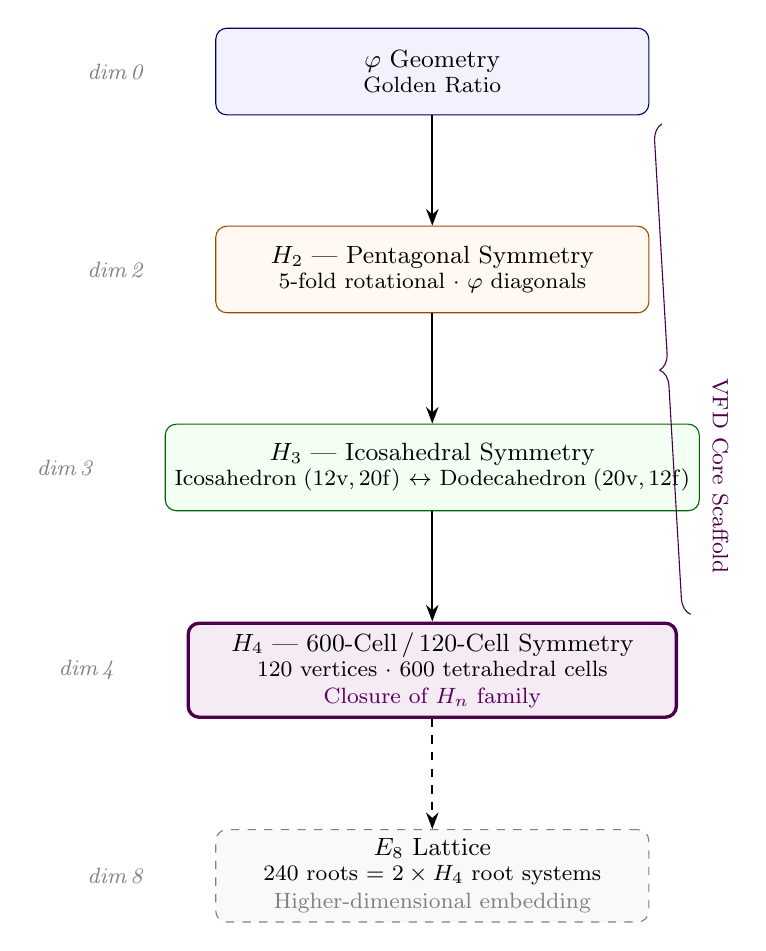
\begin{tikzpicture}[
    node distance=1.4cm,
    box/.style={draw, rounded corners=4pt, minimum width=5.5cm,
                minimum height=1.1cm, align=center, font=\small},
    arr/.style={-{Stealth[length=6pt]}, thick},
    darr/.style={-{Stealth[length=6pt]}, thick, dashed},
    lbl/.style={font=\footnotesize\itshape, text=gray}
  ]

  \node[box, fill=blue!5, draw=blue!40!black]
    (phi) {$\vphi$ Geometry\\[-2pt]
           {\footnotesize Golden Ratio}};

  \node[box, below=of phi, fill=orange!5, draw=orange!60!black]
    (h2)  {$\Htwo$ --- Pentagonal Symmetry\\[-2pt]
           {\footnotesize 5-fold rotational $\cdot$ $\vphi$ diagonals}};

  \node[box, below=of h2, fill=green!5, draw=green!40!black]
    (h3)  {$\Hthree$ --- Icosahedral Symmetry\\[-2pt]
           {\footnotesize Icosahedron\;(12v,\,20f)
            $\leftrightarrow$ Dodecahedron\;(20v,\,12f)}};

  \node[box, below=of h3, fill=violet!8, draw=violet!60!black,
        line width=1.2pt, minimum width=6.2cm]
    (h4)  {$\Hfour$ --- 600-Cell\,/\,120-Cell Symmetry\\[-2pt]
           {\footnotesize 120 vertices $\cdot$ 600 tetrahedral cells}\\[-1pt]
           {\footnotesize\color{violet!70!black}
            Closure of $H_n$ family}};

  \node[box, below=of h4, fill=gray!5, draw=gray, dashed]
    (e8)  {$\Eeight$ Lattice\\[-2pt]
           {\footnotesize 240 roots $=$ $2 \times \Hfour$ root systems}\\[-1pt]
           {\footnotesize\color{gray}
            Higher-dimensional embedding}};

  % Arrows
  \draw[arr] (phi) -- (h2);
  \draw[arr] (h2)  -- (h3);
  \draw[arr] (h3)  -- (h4);
  \draw[darr] (h4)  -- (e8);

  % Dimension labels
  \node[lbl, left=0.8cm of phi] {dim\,0};
  \node[lbl, left=0.8cm of h2]  {dim\,2};
  \node[lbl, left=0.8cm of h3]  {dim\,3};
  \node[lbl, left=0.8cm of h4]  {dim\,4};
  \node[lbl, left=0.8cm of e8]  {dim\,8};

  % Brace
  \draw[decorate, decoration={brace, amplitude=6pt, raise=4pt},
        violet!60!black]
    ($(h4.north east)+(0.3,0.1)$) -- ($(phi.south east)+(0.3,-0.1)$)
    node[midway, right=12pt, font=\footnotesize, violet!60!black,
         rotate=-90] {VFD Core Scaffold};

\end{tikzpicture}
\caption{The symmetry ladder underlying Vibrational Field Dynamics.  The
hierarchy begins with $\vphi$-geometry and pentagonal symmetry~($\Htwo$),
extends through the icosahedral group~$\Hthree$, and closes at the $\Hfour$
symmetry of the 600-cell.  The $\Eeight$ lattice (dashed) represents a
possible higher-dimensional symmetry embedding containing $\Hfour$ root
systems.}
\label{fig:ladder}
\end{figure}


% ══════════════════════════════════════════════════════════
\section{The 600-Cell as a Symmetry Boundary}\label{sec:600cell}
% ══════════════════════════════════════════════════════════

The 600-cell occupies a distinguished position in the classification of
regular polytopes.  It is the four-dimensional polytope with the largest
number of cells among the regular 4-polytopes and possesses the richest
symmetry structure.  In the VFD framework the 600-cell serves as the
\emph{maximal symmetry shell} within the $H_n$ Coxeter family---the closed
geometric constraint surface on which the dynamical field is defined.

% ── 3.1 ──────────────────────────────────────────────────
\subsection{Geometric Properties}

The 600-cell is a convex regular 4-polytope whose boundary consists of
600~regular tetrahedra~\cite{coxeter1991}.  Its key combinatorial data are
listed in Table~\ref{tab:600cell}.

\begin{table}[H]
\centering
\caption{Combinatorial data for the 600-cell.}
\label{tab:600cell}
\begin{tabular}{@{}lr@{}}
\toprule
Element & Count \\
\midrule
Vertices & 120 \\
Edges & 720 \\
Faces (triangles) & 1200 \\
Cells (tetrahedra) & 600 \\
\bottomrule
\end{tabular}
\end{table}

Each vertex of the 600-cell is surrounded by 12~edges and 20~tetrahedral
cells, giving it a local structure related to the icosahedron.  Indeed, the
\emph{vertex figure} of the 600-cell---the cross-section obtained by slicing
near a vertex---is a regular icosahedron~\cite{coxeter1991}.  This means that
the local neighbourhood of every vertex carries the full $\Hthree$ symmetry,
providing a direct geometric link between the three-dimensional and
four-dimensional levels of the symmetry ladder.

% ── 3.2 ──────────────────────────────────────────────────
\subsection{The \texorpdfstring{$\Hfour$}{H4} Root System}

The vertices of the 600-cell, when the polytope is centred at the origin and
inscribed in a unit sphere in~$\R^4$, form the root system of the Coxeter
group~$\Hfour$~\cite{coxeter1988,moody1993}.  This root system consists of
120~vectors.

Using the quaternion representation, the vertices of the 600-cell correspond
to the 120~elements of the \emph{binary icosahedral group}~$2I$, a double
cover of the icosahedral rotation group~\cite{conway2003}.  These 120 unit
quaternions can be partitioned as:
\begin{itemize}[nosep]
  \item 24~vertices forming a 24-cell (corresponding to the binary
    tetrahedral group), and
  \item 96~vertices forming the remaining shell.
\end{itemize}

The coordinates of the 120~vertices can be written explicitly using $\vphi$
and its conjugate $\hat\vphi = (1-\sqrt{5}\,)/2 = -1/\vphi$.  Representative
vertex coordinates include permutations and even sign changes
of~\cite{wilson2009}:
\begin{equation}\label{eq:600cell_coords}
  \tfrac{1}{2}(\pm 1,\,\pm 1,\,\pm 1,\,\pm 1),
  \qquad
  (0,\,0,\,0,\,\pm 1),
  \qquad
  \tfrac{1}{2}(\pm\vphi,\,\pm 1,\,\pm\hat\vphi,\,0).
\end{equation}

% ── 3.3 ──────────────────────────────────────────────────
\subsection{Graph Structure}

For the purposes of defining a discrete field theory, the relevant structure
is the \emph{graph} of the 600-cell.  Two vertices are connected by an edge if
and only if they are nearest neighbours in the polytope.  Each vertex has
exactly 12~nearest neighbours, giving the 600-cell graph a regular valency
of~12.

The adjacency structure of this graph encodes the local symmetry constraints
that any field defined on the vertices must respect.  The 600-cell graph is
\emph{vertex-transitive} (all vertices are equivalent under the symmetry
group) and \emph{edge-transitive}, ensuring that the constraint structure is
uniform across the entire shell.

% ── 3.4 ──────────────────────────────────────────────────
\subsection{Local Icosahedral Structure}\label{sec:local_ico}

An important structural feature of the 600-cell graph is that the
\emph{vertex figure} at each vertex is an icosahedron~\cite{coxeter1991}.
Equivalently, the 12~nearest neighbours of any vertex are arranged in the
geometry of the icosahedral symmetry group~$\Hthree$.  This means that the
prototype VFD dynamics combines two distinct layers of symmetry:

\begin{itemize}[nosep]
  \item \textbf{Global $\Hfour$ closure} at the level of the full 600-cell
    shell (120~vertices, $|H_4|=14\,400$).
  \item \textbf{Local $\Hthree$ coupling} at the level of each vertex
    neighbourhood (12~neighbours arranged as an icosahedron).
\end{itemize}

For the graph Laplacian, the update rule at vertex~$i$ depends entirely on
the neighbour set~$N(i)$.  Because those 12~neighbours carry icosahedral
symmetry, every local coupling step is effectively an icosahedral averaging
operation.  The field does not oscillate on an arbitrary 12-regular graph; it
oscillates on a graph whose local shell at every site is an icosahedron.

This two-layer structure---global $\Hfour$, local $\Hthree$---plausibly
contributes to the strong compression and regularity of the Laplacian
spectrum computed in Section~\ref{sec:spectrum}.  In particular, the
appearance of the square-degeneracy sequence $(\ell+1)^2$ in the low-lying
eigenvalues (Table~\ref{tab:spectrum}) is consistent with the fact that the
600-cell vertices lie on~$S^3$, while the icosahedral local geometry ensures
that the discrete graph captures important features of the continuous
symmetry at short range.

% ── Figure: Local icosahedral vertex figure ──────────────
\begin{figure}[H]
\centering
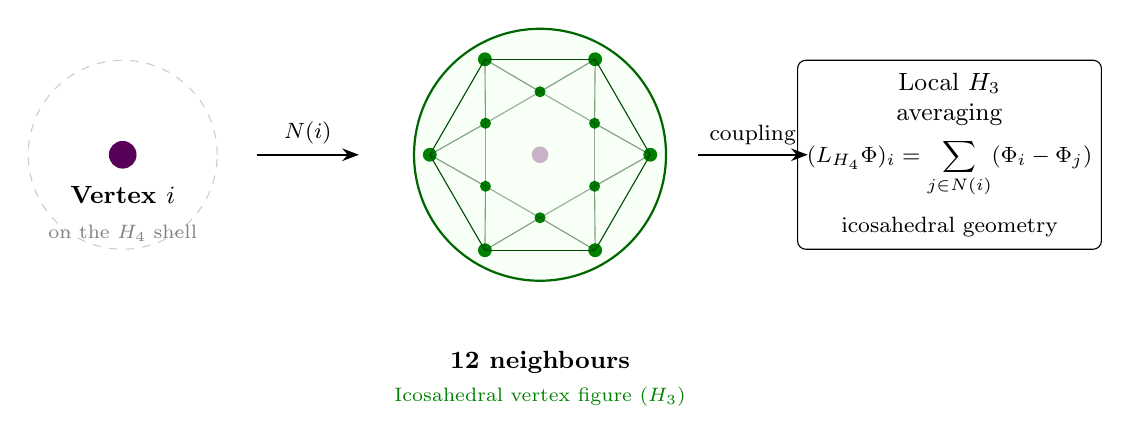
\begin{tikzpicture}[
    arr/.style={-{Stealth[length=6pt]}, thick},
  ]

  % Left: single vertex
  \begin{scope}[shift={(-3.5,0)}]
    \fill[violet!70!black] (0,0) circle (5pt);
    \node[font=\small\bfseries, below=8pt] at (0,0) {Vertex $i$};
    \draw[gray!40, dashed] (0,0) circle (1.2cm);
    \node[font=\scriptsize, text=gray, below=22pt] at (0,0)
      {on the $\Hfour$ shell};
  \end{scope}

  % Arrow
  \draw[arr] (-1.8,0) -- (-0.5,0)
    node[midway, above, font=\footnotesize] {$N(i)$};

  % Right: 12-neighbour icosahedral shell
  \begin{scope}[shift={(1.8,0)}]
    \draw[green!40!black, thick, fill=green!3] (0,0) circle (1.6cm);

    % 12 vertices of icosahedron (projected)
    \foreach \a [count=\i] in {0,60,120,180,240,300} {
      \fill[green!50!black] (\a:1.4) circle (2.5pt);
    }
    \foreach \a [count=\i] in {30,90,150,210,270,330} {
      \fill[green!50!black] (\a:0.8) circle (2pt);
    }

    % Icosahedral edges (subset)
    \foreach \a in {0,60,120,180,240,300} {
      \pgfmathsetmacro{\b}{\a+60}
      \draw[green!30!black, thin] (\a:1.4) -- (\b:1.4);
      \draw[green!25!black, thin, opacity=0.5]
        (\a:1.4) -- ({\a+30}:0.8);
      \draw[green!25!black, thin, opacity=0.5]
        (\a:1.4) -- ({\a-30}:0.8);
    }
    \foreach \a in {30,90,150,210,270,330} {
      \pgfmathsetmacro{\b}{\a+60}
      \draw[green!20!black, thin, opacity=0.4] (\a:0.8) -- (\b:0.8);
    }

    % Central vertex (faded)
    \fill[violet!70!black, opacity=0.3] (0,0) circle (3pt);

    \node[font=\small\bfseries, below=22pt] at (0,-1.6)
      {12 neighbours};
    \node[font=\scriptsize, text=green!50!black, below=35pt] at (0,-1.6)
      {Icosahedral vertex figure ($\Hthree$)};
  \end{scope}

  % Arrow to interpretation
  \draw[arr] (3.8,0) -- (5.2,0)
    node[midway, above, font=\footnotesize] {coupling};

  % Right: interpretation box
  \begin{scope}[shift={(7,0)}]
    \node[draw, rounded corners=3pt, minimum width=3cm,
          minimum height=2.4cm, align=center, font=\small] at (0,0)
      {Local $\Hthree$\\averaging\\[4pt]
       {\footnotesize $(\Lmat\Phi)_i = \displaystyle\sum_{j\in N(i)}
        (\Phi_i - \Phi_j)$}\\[6pt]
       {\footnotesize icosahedral geometry}};
  \end{scope}

\end{tikzpicture}
\caption{Local geometry of the 600-cell graph.  Each vertex~$i$ has
12~nearest neighbours arranged as an icosahedron (the vertex figure).  The
graph Laplacian couples the field through repeated local $\Hthree$-symmetric
averaging, embedded within the globally $\Hfour$-symmetric shell.}
\label{fig:local_ico}
\end{figure}

% ── 3.5 ──────────────────────────────────────────────────
\subsection{The 600-Cell as a Closed Constraint Shell}

The combination of these properties---maximal symmetry within the $H_n$
family, a well-defined root system, icosahedral vertex figures, and a regular
graph structure---makes the 600-cell a natural candidate for a geometric
constraint boundary.  In the VFD framework we interpret the 600-cell as a
\emph{closed symmetry shell}: a maximal geometric structure that constrains
the modes of a field defined on its vertices.

The maximality property is essential.  Because $\Hfour$ is the terminal member
of the non-crystallographic Coxeter family, the 600-cell is not a truncation
or approximation of a higher-dimensional object within this family.  It is the
\emph{final} regular structure, and its symmetries define the maximal set of
geometric constraints available from the $\vphi$-based hierarchy.

The role of the 600-cell is purely geometric: it defines a closed
symmetry-constrained graph on which the field dynamics are formulated.
No additional physical assumptions are required at this stage.

% ── Figure 3: H4 Root Structure ──────────────────────────
\begin{figure}[H]
\centering
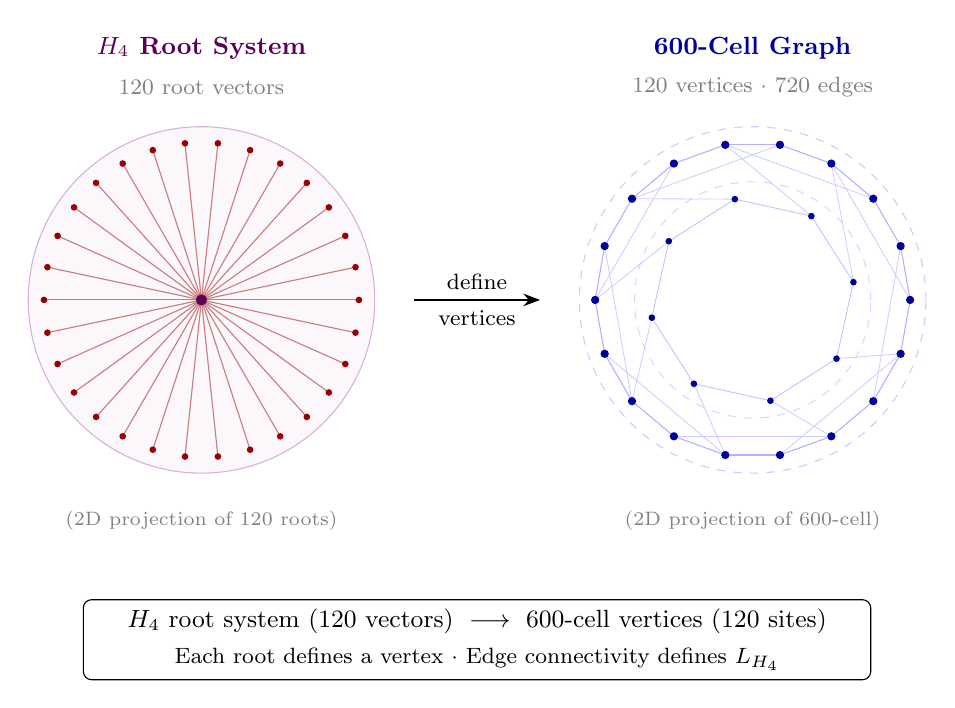
\begin{tikzpicture}[
    arr/.style={-{Stealth[length=6pt]}, thick},
  ]

  % Left: Root system
  \begin{scope}[shift={(-3.5,0)}]
    \node[font=\small\bfseries, text=violet!70!black] at (0,3.2)
      {$\Hfour$ Root System};
    \node[font=\footnotesize, text=gray] at (0,2.7) {120 root vectors};

    \draw[violet!30, fill=violet!3] (0,0) circle (2.2cm);

    % Radial root lines
    \foreach \a in {0,12,...,348} {
      \draw[red!60!black, line width=0.4pt, opacity=0.5]
        (0,0) -- (\a:2.0);
      \fill[red!60!black] (\a:2.0) circle (1.2pt);
    }
    \fill[violet!70!black] (0,0) circle (2pt);

    \node[font=\scriptsize, text=gray] at (0,-2.8)
      {(2D projection of 120 roots)};
  \end{scope}

  % Arrow
  \draw[arr] (-0.8,0) -- (0.8,0)
    node[midway, above, font=\footnotesize] {define}
    node[midway, below, font=\footnotesize] {vertices};

  % Right: 600-cell graph
  \begin{scope}[shift={(3.5,0)}]
    \node[font=\small\bfseries, text=blue!60!black] at (0,3.2)
      {600-Cell Graph};
    \node[font=\footnotesize, text=gray] at (0,2.7)
      {120 vertices $\cdot$ 720 edges};

    \draw[blue!20, dashed] (0,0) circle (2.2cm);
    \draw[blue!15, dashed] (0,0) circle (1.5cm);

    % Outer ring vertices + edges (subset)
    \foreach \a [count=\i] in {0,20,...,340} {
      \coordinate (o\i) at (\a:2.0);
    }
    \foreach \i in {1,...,18} {
      \pgfmathtruncatemacro{\next}{mod(\i,18)+1}
      \draw[blue!30, line width=0.4pt] (o\i) -- (o\next);
    }
    % Cross edges
    \foreach \i in {1,3,...,17} {
      \pgfmathtruncatemacro{\skip}{mod(\i+2,18)+1}
      \draw[blue!20, line width=0.3pt] (o\i) -- (o\skip);
    }
    % Inner ring
    \foreach \a [count=\i] in {10,55,100,145,190,235,280,325} {
      \coordinate (in\i) at (\a:1.3);
    }
    \foreach \i in {1,...,8} {
      \pgfmathtruncatemacro{\next}{mod(\i,8)+1}
      \draw[blue!25, line width=0.3pt] (in\i) -- (in\next);
    }
    % Radial connections
    \foreach \i in {1,...,8} {
      \pgfmathtruncatemacro{\oi}{mod(2*\i+1,18)+1}
      \draw[blue!20, line width=0.3pt] (in\i) -- (o\oi);
    }
    % Dots
    \foreach \i in {1,...,18} {
      \fill[blue!60!black] (o\i) circle (1.5pt);
    }
    \foreach \i in {1,...,8} {
      \fill[blue!60!black] (in\i) circle (1.2pt);
    }

    \node[font=\scriptsize, text=gray] at (0,-2.8)
      {(2D projection of 600-cell)};
  \end{scope}

  % Bottom box
  \node[draw, rounded corners=3pt, minimum width=10cm, minimum height=1cm,
        align=center, font=\small, anchor=north] at (0,-3.8)
    {$\Hfour$ root system (120 vectors)
     $\;\longrightarrow\;$
     600-cell vertices (120 sites)\\[2pt]
     {\footnotesize Each root defines a vertex $\cdot$
      Edge connectivity defines $\Lmat$}};

\end{tikzpicture}
\caption{The $\Hfour$ root system (left) consists of 120~vectors whose
endpoints define the vertices of the 600-cell (right).  The edge connectivity
of the 600-cell graph defines the adjacency structure used to construct the
graph Laplacian~$\Lmat$.}
\label{fig:h4roots}
\end{figure}


% ══════════════════════════════════════════════════════════
\section{Field Definition on the \texorpdfstring{$\Hfour$}{H4} Manifold}
\label{sec:field}
% ══════════════════════════════════════════════════════════

% ── 4.1 ──────────────────────────────────────────────────
\subsection{The Continuous Setting}

In the most general formulation one considers a real scalar field defined on a
manifold associated with the $\Hfour$ symmetry group.  Let $\mathcal{M}$
denote the symmetry manifold---for instance, the orbit space of a point under
the action of~$\Hfour$, or a smooth manifold whose isometry group
contains~$\Hfour$.  The field is a smooth function
\begin{equation}\label{eq:field_cont}
  \Phi : \mathcal{M} \times \R \longrightarrow \R
\end{equation}
where the first argument represents position on the manifold and the second
represents time.  The dynamics of~$\Phi$ are governed by a wave-type equation
incorporating the geometric structure of $\mathcal{M}$ through its
Laplace--Beltrami operator.

However, the continuous setting requires a precise specification of
$\mathcal{M}$ as a Riemannian manifold, which introduces additional choices
(metric, topology) beyond the discrete symmetry data.  For the purposes of
establishing the foundational framework we adopt a discrete approach that
depends only on the combinatorial structure of the 600-cell.

% ── 4.2 ──────────────────────────────────────────────────
\subsection{The Discrete Field on the 600-Cell Graph}

Let $V(\Hfour)$ denote the set of 120~vertices of the 600-cell.  We define a
real scalar field on this vertex set:
\begin{equation}\label{eq:field_disc}
  \Phi_i(t), \qquad i \in V(\Hfour),
  \quad \lvert V(\Hfour)\rvert = 120
\end{equation}
where $i$ indexes the vertices and $t$ denotes time.  The field value
$\Phi_i(t)$ represents the amplitude of the field at vertex~$i$ at time~$t$.
The state of the system at any time is therefore a vector in~$\R^{120}$.

The space of all such field configurations inherits the symmetry of the
600-cell: the Coxeter group $\Hfour$ acts on~$\R^{120}$ by permuting the
vertex labels according to the symmetries of the polytope.  This action
decomposes the space of field configurations into irreducible representations
of~$\Hfour$, a fact that will be central to the analysis of eigenmodes.

% ── 4.3 ──────────────────────────────────────────────────
\subsection{The \texorpdfstring{$\Hfour$}{H4} Graph Laplacian}

To express the symmetry-constrained coupling between field values at
neighbouring vertices, we introduce the graph Laplacian associated with the
600-cell connectivity structure.

\begin{quote}
\textbf{Definition.}\; Let $G = (V, E)$ be the graph of the 600-cell, where
$V = V(\Hfour)$ is the vertex set and $E$ is the edge set.  For a function
$\Phi : V \to \R$, the \emph{graph Laplacian} is defined by
\begin{equation}\label{eq:laplacian}
  \boxed{(\Lmat\,\Phi)_i
    \;=\; \sum_{j \in N(i)} \bigl(\Phi_i - \Phi_j\bigr)}
\end{equation}
where $N(i)$ denotes the set of vertices adjacent to vertex~$i$ in the graph.
\end{quote}

Since the 600-cell graph is 12-regular (every vertex has exactly 12
neighbours), the Laplacian can also be written in matrix form as
\begin{equation}\label{eq:laplacian_matrix}
  \Lmat = 12\,I - A
\end{equation}
where $A$ is the $120 \times 120$ adjacency matrix of the 600-cell graph and
$I$ is the identity matrix.

The graph Laplacian is a symmetric positive semi-definite matrix.  Its null
space is spanned by the constant vector (the trivial mode), and its nonzero
eigenvalues encode the connectivity structure of the graph.  Because the
600-cell graph is vertex-transitive under~$\Hfour$, the eigenspaces
of~$\Lmat$ are invariant subspaces of the permutation representation
of~$\Hfour$, ensuring that the eigenvalue decomposition respects the symmetry
of the polytope.

% ── 4.4 ──────────────────────────────────────────────────
\subsection{Prototype VFD Field Equation}

The simplest dynamical model consistent with these constraints is a nonlinear
oscillator system defined on the graph.  The prototype VFD field equation is
\begin{equation}\label{eq:vfd}
  \boxed{\ddot{\Phi}_i
    + \omega_0^2\,\Phi_i
    + \lambda\,(\Lmat\,\Phi)_i
    + \beta\,\Phi_i^3 = 0}
\end{equation}
where:
\begin{itemize}[nosep]
  \item $\omega_0$ is a baseline oscillation frequency, providing a restoring
    force independent of geometry;
  \item $\lambda$ is a coupling constant governing the strength of geometric
    interactions between neighbouring vertices;
  \item $\beta$ is a nonlinear coefficient controlling the amplitude-dependent
    self-interaction of the field;
  \item the overdot denotes differentiation with respect to time.
\end{itemize}

This equation is introduced as a prototype dynamical system.  No claim
is made that it represents a fundamental physical field equation.  It
represents a system of 120~coupled nonlinear oscillators constrained by
the symmetry geometry of the 600-cell.  The Laplacian term
ensures that the evolution of the field respects the adjacency relations
defined by the $\Hfour$ structure, while the nonlinear term allows the
formation of stable localised modes.

\begin{table}[H]
\centering
\caption{Terms in the prototype VFD field equation.}
\label{tab:terms}
\begin{tabular}{@{}ll@{}}
\toprule
Term & Physical Role \\
\midrule
$\ddot{\Phi}_i$ & Inertia / oscillatory dynamics \\
$\omega_0^2\,\Phi_i$ & Baseline restoring force \\
$\lambda\,(\Lmat\,\Phi)_i$ & Geometric coupling to neighbours \\
$\beta\,\Phi_i^3$ & Nonlinear self-interaction \\
\bottomrule
\end{tabular}
\end{table}

The equation is Hamiltonian, derivable from the energy functional
\begin{equation}\label{eq:hamiltonian}
  H = \sum_{i} \left[
    \frac{1}{2}\dot{\Phi}_i^2
    + \frac{\omega_0^2}{2}\Phi_i^2
    + \frac{\lambda}{4}\sum_{j \in N(i)}(\Phi_i - \Phi_j)^2
    + \frac{\beta}{4}\Phi_i^4
  \right].
\end{equation}
This ensures energy conservation and provides a variational foundation for the
dynamics.


% ══════════════════════════════════════════════════════════
\section{Resonant Eigenmodes}\label{sec:eigenmodes}
% ══════════════════════════════════════════════════════════

% ── 5.1 ──────────────────────────────────────────────────
\subsection{The Linear Eigenmode Problem}

To understand the basic resonant structure of the system we first consider the
linearised version obtained by setting $\beta = 0$:
\begin{equation}\label{eq:linear}
  \ddot{\Phi}_i
  + \omega_0^2\,\Phi_i
  + \lambda\,(\Lmat\,\Phi)_i = 0.
\end{equation}
Seeking harmonic solutions of the form
$\Phi_i(t) = A_i\,e^{i\Omega t}$,
we obtain the matrix eigenvalue problem
\begin{equation}\label{eq:eigenvalue}
  \boxed{(\omega_0^2\,I + \lambda\,\Lmat)\,A = \Omega^2\,A}
\end{equation}

This is a standard symmetric eigenvalue problem for the $120 \times 120$
matrix $M = \omega_0^2 I + \lambda\Lmat$.  Since $\Lmat$ is positive
semi-definite with eigenvalues
$0 = \mu_1 \le \mu_2 \le \cdots \le \mu_{120}$,
the resonance frequencies are
\begin{equation}\label{eq:frequencies}
  \Omega_k^2 = \omega_0^2 + \lambda\,\mu_k, \qquad k = 1,\ldots,120.
\end{equation}
The eigenvectors $A^{(k)}$ represent the symmetry-constrained normal modes of
the field on the $\Hfour$ manifold.  Each eigenmode corresponds to a
standing-wave configuration defined over the vertices of the 600-cell.
The eigenvalues arise entirely from the combinatorial structure of the
600-cell graph and do not depend on any physical parameter choices.

% ── 5.2 ──────────────────────────────────────────────────
\subsection{Symmetry Structure of the Laplacian}\label{sec:sym_laplacian}

The structure of the Laplacian spectrum is strongly constrained by the
symmetry of the 600-cell graph.  Before presenting the explicit computation we
establish the group-theoretic reason for this constraint.

Let $G = (V, E)$ denote the graph of the 600-cell and let $\Lmat$ be its
graph Laplacian.  The Coxeter group $\Hfour$ acts on the vertex set~$V$ by
permuting vertices through the symmetries of the polytope.

\medskip
\noindent\textbf{Proposition.}\;
\textit{The graph Laplacian $\Lmat$ commutes with the action of the Coxeter
group $\Hfour$ on the vertex space~$\R^{120}$:}
\begin{equation}\label{eq:commutation}
  g\,\Lmat = \Lmat\,g \qquad \forall\, g \in \Hfour.
\end{equation}

\begin{proof}
The adjacency relation of the 600-cell graph is preserved by every symmetry of
the polytope.  Since the Laplacian is defined solely in terms of this adjacency
relation,
\[
  (\Lmat\,\Phi)_i = \sum_{j \in N(i)} (\Phi_i - \Phi_j),
\]
the action of any symmetry $g \in \Hfour$ simply permutes the vertex labels
while leaving the connectivity structure invariant.  Therefore
$g(\Lmat\,\Phi) = \Lmat\,(g\Phi)$, establishing the commutation
relation~\eqref{eq:commutation}.
\end{proof}

\noindent\textbf{Consequence.}\;
Because $\Lmat$ commutes with the $\Hfour$ action, the vertex space
decomposes into invariant subspaces corresponding to irreducible
representations of~$\Hfour$:
\begin{equation}\label{eq:decomp}
  \R^{120} = \bigoplus_{\alpha} V_\alpha.
\end{equation}
Each eigenspace of the Laplacian must lie within one of these symmetry
sectors.  The multiplicities of the eigenvalues are consequently constrained
by the representation theory of~$\Hfour$, and the degeneracy structure of the
spectrum is \emph{not} accidental but follows necessarily from the symmetry of
the underlying graph.

This observation means that the spectral structure reported below is governed
by
\[
  \Hfour\text{ symmetry}
  \;\longrightarrow\;
  \text{representation decomposition}
  \;\longrightarrow\;
  \text{degenerate eigenmode sectors}
\]
rather than being a numerical curiosity of a particular graph.

% ── 5.3 ──────────────────────────────────────────────────
\subsection{First-Pass Spectrum of the 600-Cell Graph Laplacian}
\label{sec:spectrum}

As a first explicit computation within the proposed $\Hfour$-constrained field
model, we determine the spectrum of the 600-cell graph Laplacian
$\Lmat = 12I - A$, where $A$ is the adjacency matrix of the 600-cell graph.
Using the standard 120-vertex realisation and nearest-neighbour edge
connectivity, the graph is confirmed to be 12-regular with 720~edges.

The Laplacian spectrum contains only \textbf{nine distinct eigenvalues},
listed in ascending order with their multiplicities in
Table~\ref{tab:spectrum}.

\begin{table}[H]
\centering
\caption{Eigenvalues and multiplicities of the 600-cell graph Laplacian
$\Lmat = 12I - A$.  The nine distinct eigenvalues compress
120~degrees of freedom into nine resonance
sectors.\protect\footnote{The exceptional regularity of the spectrum
suggests that it arises from the distance-regular structure and symmetry
algebra of the 600-cell graph rather than from generic graph-theoretic
behaviour.}}
\label{tab:spectrum}
\begin{tabular}{@{}crrl@{}}
\toprule
Sector $k$ & Eigenvalue $\mu_k$ & Multiplicity $d_k$ & Note \\
\midrule
1 & $0$                              & 1  & $= 1^2$ \\
2 & $9 - 3\sqrt{5} \approx 2.292$   & 4  & $= 2^2$ \\
3 & $10 - 2\sqrt{5} \approx 5.528$  & 9  & $= 3^2$ \\
4 & $9$                              & 16 & $= 4^2$ \\
5 & $12$                             & 25 & $= 5^2$ \\
6 & $14$                             & 36 & $= 6^2$ \\
7 & $10 + 2\sqrt{5} \approx 14.472$ & 9  & \\
8 & $15$                             & 16 & \\
9 & $9 + 3\sqrt{5} \approx 15.708$  & 4  & \\
\bottomrule
\addlinespace
\multicolumn{4}{@{}l}{\footnotesize
  $\sum d_k = 1+4+9+16+25+36+9+16+4 = 120$. \quad
  Eigenvalues involving $\sqrt{5}$ lie in $\Q(\sqrt{5}\,)$.}
\end{tabular}
\end{table}

The spectrum was obtained by constructing the adjacency matrix of the
600-cell graph using the vertex coordinates and inner-product criterion
described in Appendix~\ref{app:construction}, then performing symmetric
eigendecomposition of the Laplacian matrix $\Lmat = 12I - A$ using standard
numerical linear algebra methods.

This result is noteworthy for two reasons.  First, the 120-dimensional system
collapses into only nine distinct resonance levels, indicating a highly
compressed mode structure.  Second, the first six multiplicities form the
perfect-square sequence
\begin{equation}\label{eq:squares}
  d_1,\ldots,d_6 \;=\; 1^2,\; 2^2,\; 3^2,\; 4^2,\; 5^2,\; 6^2
\end{equation}
which is characteristic of the degeneracy pattern of harmonic analysis on
the 3-sphere~$S^3$, where the eigenspaces of the Laplace--Beltrami operator
have dimension $(\ell+1)^2$ for angular momentum quantum number~$\ell$.  The
fact that this pattern persists for the first six sectors of the discrete
600-cell graph suggests that the low-lying modes closely approximate the
continuous hyperspherical harmonics, with deviations appearing only in the
upper part of the spectrum.  This multiplicity structure is highly
non-generic and does not occur in typical regular graphs of comparable
size and degree.

The four irrational eigenvalues---$9 \pm 3\sqrt{5}$ and
$10 \pm 2\sqrt{5}$---take values in the number field~$\Q(\sqrt{5}\,)$,
confirming the algebraic connection to the golden ratio that pervades the
$H_n$ symmetry family.  The remaining five eigenvalues
($0, 9, 12, 14, 15$) are rational integers.  Note that the irrational
eigenvalues appear in conjugate pairs, as expected from the Galois symmetry of
$\Q(\sqrt{5}\,)/\Q$.

Within the present framework this spectrum constitutes the first concrete
output of the VFD prototype model: a discrete hierarchy of
symmetry-constrained standing-wave sectors on the 600-cell graph.  While no
direct physical identification is claimed at this stage, the existence of such
a structured spectral organisation supports the hypothesis that the $\Hfour$
geometry provides a nontrivial and highly ordered constraint space for
resonant structure formation.

% ── Figure 5: Spectrum ───────────────────────────────────
\begin{figure}[H]
\centering
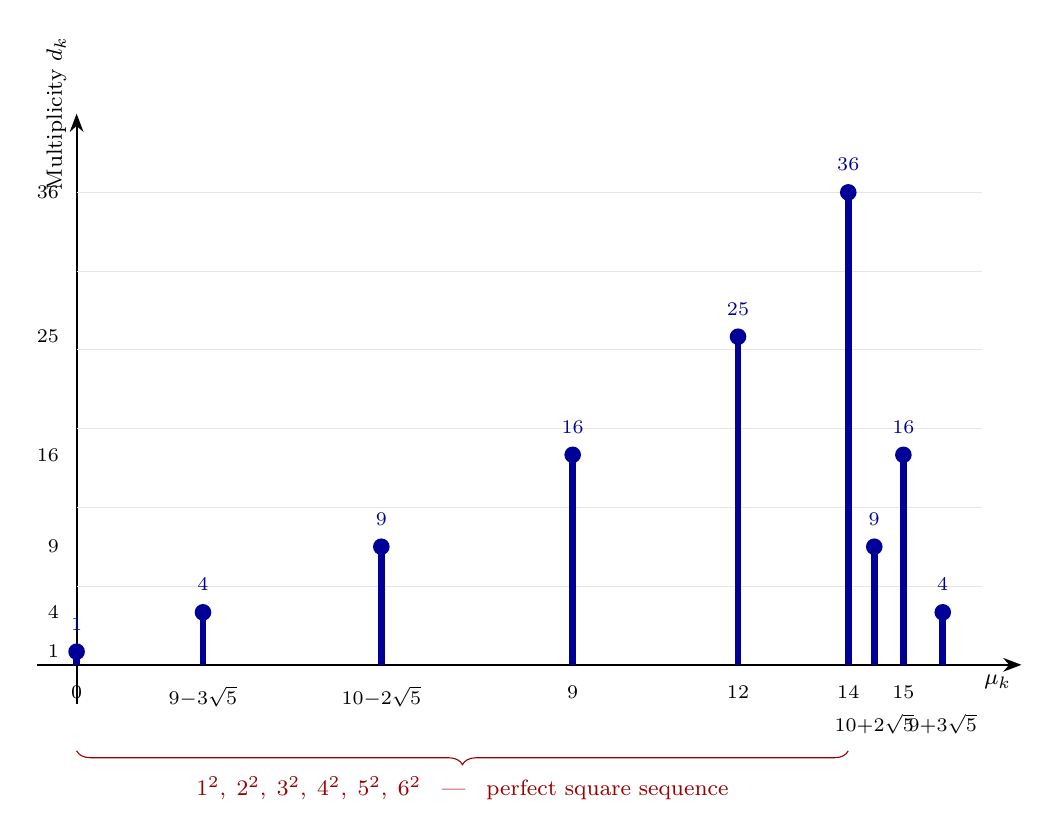
\begin{tikzpicture}[
    every node/.style={font=\small},
  ]

  % Axes
  \draw[thick, -{Stealth}] (-0.5,0) -- (12,0)
    node[below left, font=\footnotesize] {$\mu_k$};
  \draw[thick, -{Stealth}] (0,-0.5) -- (0,7)
    node[above left, font=\footnotesize, rotate=90, anchor=south]
    {Multiplicity $d_k$};

  % Grid lines
  \foreach \y in {1,...,6} {
    \draw[gray!20] (0,\y) -- (11.5,\y);
  }

  % Scale: x = mu * 11/15.708 ≈ mu * 0.7,  y = d/6
  % mu:  0     2.292  5.528   9     12     14     14.472  15     15.708
  % x:   0     1.605  3.870   6.3   8.4    9.8    10.130  10.5   11.0
  % d:   1     4      9       16    25     36     9       16     4
  % y:   0.167 0.667  1.5     2.667 4.167  6.0    1.5     2.667  0.667

  % Stems
  \foreach \mx/\my/\d in {
    0/0.167/1,
    1.605/0.667/4,
    3.870/1.5/9,
    6.300/2.667/16,
    8.400/4.167/25,
    9.800/6.0/36,
    10.130/1.5/9,
    10.500/2.667/16,
    11.000/0.667/4
  } {
    \draw[blue!60!black, line width=2.5pt] (\mx,0) -- (\mx,\my);
    \fill[blue!60!black] (\mx,\my) circle (3pt);
    \node[above, font=\scriptsize, blue!60!black] at (\mx,\my+0.15)
      {\d};
  }

  % x-axis eigenvalue labels
  \node[below, font=\scriptsize] at (0,-0.15) {$0$};
  \node[below, font=\scriptsize, align=center] at (1.605,-0.15)
    {$9{-}3\sqrt{5}$};
  \node[below, font=\scriptsize, align=center] at (3.870,-0.15)
    {$10{-}2\sqrt{5}$};
  \node[below, font=\scriptsize] at (6.300,-0.15) {$9$};
  \node[below, font=\scriptsize] at (8.400,-0.15) {$12$};
  \node[below, font=\scriptsize] at (9.800,-0.15) {$14$};
  \node[below, font=\scriptsize, align=center] at (10.130,-0.5)
    {$10{+}2\sqrt{5}$};
  \node[below, font=\scriptsize] at (10.500,-0.15) {$15$};
  \node[below, font=\scriptsize, align=center] at (11.000,-0.5)
    {$9{+}3\sqrt{5}$};

  % y-axis labels
  \foreach \y/\v in {0.167/1, 0.667/4, 1.5/9, 2.667/16, 4.167/25, 6.0/36} {
    \node[left, font=\scriptsize] at (-0.1,\y) {\v};
  }

  % Annotation: square sequence bracket
  \draw[decorate, decoration={brace, amplitude=5pt, mirror, raise=14pt},
        red!60!black]
    (0,-0.6) -- (9.800,-0.6)
    node[midway, below=20pt, font=\footnotesize, red!60!black]
    {$1^2,\; 2^2,\; 3^2,\; 4^2,\; 5^2,\; 6^2$
     \;\;---\;\; perfect square sequence};

\end{tikzpicture}
\caption{Distinct eigenvalues of the 600-cell graph Laplacian~$\Lmat$ and
their multiplicities.  The spectrum compresses 120~degrees of freedom into
nine resonance sectors.  The first six multiplicities (brace) follow the
perfect-square sequence~$n^2$, mirroring the degeneracy pattern of
hyperspherical harmonics on~$S^3$.}
\label{fig:spectrum}
\end{figure}


% ── 5.3 ──────────────────────────────────────────────────
\subsection{Symmetry and Degeneracy}

The eigenvalue spectrum of $\Lmat$ is highly structured due to the symmetry of
the 600-cell graph.  Because the graph is vertex-transitive under the action
of~$\Hfour$, the eigenspaces of the Laplacian decompose into irreducible
representations of~$\Hfour$~\cite{chung1997}.  This means:

\begin{enumerate}[nosep]
  \item \textbf{Eigenvalues are highly degenerate.}  The 120~modes do not
    yield 120~distinct frequencies; they organise into a much smaller number of
    distinct eigenvalues, each with a degeneracy equal to the dimension of the
    corresponding irreducible representation.

  \item \textbf{The degeneracy pattern is determined by representation
    theory.}  The specific multiplicities follow from the decomposition of the
    120-dimensional permutation representation of~$\Hfour$ into irreducible
    components.

  \item \textbf{The lowest mode is always trivial.}  The constant eigenvector
    (all components equal) corresponds to eigenvalue $\mu_1 = 0$ with
    degeneracy~1.
\end{enumerate}

The spectral structure of the 600-cell graph Laplacian has been studied in the
context of algebraic graph theory~\cite{brouwer2012}.  The eigenvalues reflect the algebraic structure associated with the
$\vphi$-based symmetry family, with several taking values in the number
field~$\Q(\sqrt{5}\,)$.

% ── 5.3 ──────────────────────────────────────────────────
\subsection{Mode Classification}

The eigenmodes can be classified according to their transformation properties
under~$\Hfour$:

\begin{itemize}[nosep]
  \item \textbf{Trivial mode} ($\Omega_1$): the uniform configuration where
    all vertices oscillate in phase.  This is the lowest-frequency mode.
  \item \textbf{Vector modes} (low~$\Omega$): modes transforming as the
    fundamental 4-dimensional representation of~$\Hfour$.  These are analogous
    to dipole oscillations on a sphere.
  \item \textbf{Higher harmonics}: modes transforming as higher irreducible
    representations, with increasingly complex spatial patterns on the
    600-cell graph.
  \item \textbf{Highest mode} ($\Omega_{\max}$): the mode with maximum
    variation between neighbouring vertices, corresponding to the largest
    Laplacian eigenvalue.
\end{itemize}

The progression from low to high modes represents increasing geometric
complexity of the standing-wave pattern on the symmetry shell.  In the VFD
interpretation the low-lying modes with the simplest spatial structure are the
primary candidates for stable physical configurations.

% ── 5.4 ──────────────────────────────────────────────────
\subsection{Comparison with Spherical Harmonics}

The eigenmode decomposition on the 600-cell graph is the discrete analogue of
the spherical harmonic decomposition of the Laplacian on~$S^2$ or, more
precisely, the harmonic analysis on the 3-sphere~$S^3$ (since the vertices of
the 600-cell lie on $S^3 \subset \R^4$).

On the continuous 3-sphere the eigenvalues of the Laplace--Beltrami operator
are $\ell(\ell+2)$ with degeneracy $(\ell+1)^2$, and the eigenfunctions are
the hyperspherical harmonics~\cite{vilenkin1993}.  The 600-cell eigenmode
spectrum can be understood as a \emph{symmetry-reduced discretisation} of this
continuous spectrum: the $\Hfour$ symmetry selects a finite subset of modes
from the continuous family, and the discrete graph structure modifies the
eigenvalues from their continuous values.

This relationship provides a bridge between the discrete VFD framework and
continuous field theory on curved spaces.

% ── 5.7 ──────────────────────────────────────────────────
\subsection{Spectral Structure of the 600-Cell Graph}

The Laplacian spectrum of the 600-cell graph exhibits an
unusually high degree of algebraic structure.  In particular,
the spectrum contains only nine distinct eigenvalues across
120 degrees of freedom, and the associated multiplicities
follow the sequence
\[
1,\;4,\;9,\;16,\;25,\;36,\;9,\;16,\;4.
\]

The first six multiplicities form the perfect-square sequence
$(\ell+1)^2$, reminiscent of the degeneracy pattern of
hyperspherical harmonics on the three-sphere~$S^3$.
Furthermore, the irrational eigenvalues occur in conjugate
pairs involving $\sqrt{5}$ and therefore lie in the number
field~$\Q(\sqrt{5}\,)$, reflecting the golden-ratio
structure characteristic of the non-crystallographic Coxeter
family.

These features strongly suggest that the Laplacian spectrum
is governed by deeper algebraic constraints associated with
the symmetry and combinatorial structure of the 600-cell
graph.  In particular, the graph is distance-regular and
admits a large automorphism group inherited from the
$\Hfour$ symmetry of the polytope.  In such graphs the
adjacency and Laplacian operators belong to a small
commutative algebra generated by the graph distance
operators, leading to a correspondingly small set of
distinct eigenvalues.

The numerical results presented here therefore reflect
an underlying algebraic structure associated with the
distance-regular geometry and symmetry algebra of the 600-cell
graph, combined with the representation theory of the $\Hfour$
symmetry group.  A full analytic derivation
of the eigenvalues and multiplicities from this structure
would require a detailed analysis of the associated
Bose--Mesner algebra or related symmetry constructions and
is left for future work.


% ── Figure 2: Structure Formation ────────────────────────
\begin{figure}[H]
\centering
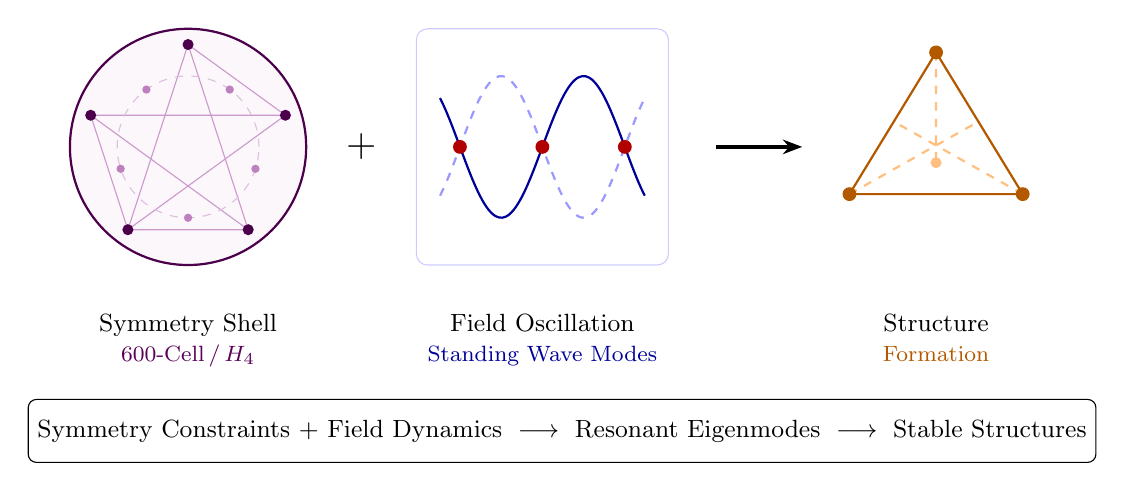
\begin{tikzpicture}[
    arr/.style={-{Stealth[length=7pt]}, very thick},
    lbl/.style={font=\small, align=center},
  ]

  % Panel 1: Symmetry Shell
  \begin{scope}[shift={(-4.5,0)}]
    \draw[violet!60!black, thick, fill=violet!3] (0,0) circle (1.5cm);
    % Icosahedral wireframe
    \foreach \a in {90,162,234,306,378} {
      \coordinate (p\a) at (\a:1.3);
    }
    \draw[violet!40, thin]
      (p90)--(p234)--(p378)--(p162)--(p306)--(p90);
    \draw[violet!40, thin]
      (p90)--(p378) (p234)--(p306) (p234)--(p162);
    \foreach \a in {90,162,234,306,378} {
      \fill[violet!60!black] (\a:1.3) circle (2pt);
    }
    \draw[violet!25, dashed, thin] (0,0) circle (0.9cm);
    \foreach \a in {54,126,198,270,342} {
      \fill[violet!50] (\a:0.9) circle (1.5pt);
    }
    \node[lbl, below] at (0,-2) {Symmetry Shell\\
      {\footnotesize\color{violet!70!black} 600-Cell\,/\,$\Hfour$}};
  \end{scope}

  % Plus
  \node[font=\Large] at (-2.3,0) {$+$};

  % Panel 2: Standing Waves
  \begin{scope}[shift={(0,0)}]
    \draw[blue!20, rounded corners=4pt]
      (-1.6,-1.5) rectangle (1.6,1.5);
    \draw[blue!60!black, thick, smooth]
      plot[domain=-1.3:1.3, samples=60]
      (\x, {0.9*sin(3*\x*180/3.14)});
    \draw[blue!40, thick, smooth, dashed]
      plot[domain=-1.3:1.3, samples=60]
      (\x, {-0.9*sin(3*\x*180/3.14)});
    % Nodes
    \foreach \x in {-1.047,0,1.047} {
      \fill[red!70!black] (\x,0) circle (2.5pt);
    }
    \node[lbl, below] at (0,-2) {Field Oscillation\\
      {\footnotesize\color{blue!60!black} Standing Wave Modes}};
  \end{scope}

  % Arrow
  \draw[arr] (2.2,0) -- (3.3,0);

  % Panel 3: Structure
  \begin{scope}[shift={(5,0)}]
    % Tetrahedron
    \draw[orange!70!black, thick]
      (0,1.2) -- (-1.1,-0.6) -- (1.1,-0.6) -- cycle;
    \draw[orange!50, thick, dashed]
      (0,1.2) -- (0,-0.2)
      (-1.1,-0.6) -- (0.5,0.3)
      (1.1,-0.6) -- (-0.5,0.3);
    \fill[orange!70!black] (0,1.2) circle (2.5pt);
    \fill[orange!70!black] (-1.1,-0.6) circle (2.5pt);
    \fill[orange!70!black] (1.1,-0.6) circle (2.5pt);
    \fill[orange!50] (0,-0.2) circle (2pt);
    \node[lbl, below] at (0,-2) {Structure\\
      {\footnotesize\color{orange!70!black} Formation}};
  \end{scope}

  % Bottom equation
  \node[draw, rounded corners=3pt, minimum width=11cm,
        minimum height=0.8cm, anchor=north, font=\small]
    at (0.25,-3.2)
    {Symmetry Constraints $+$ Field Dynamics
     $\;\longrightarrow\;$ Resonant Eigenmodes
     $\;\longrightarrow\;$ Stable Structures};

\end{tikzpicture}
\caption{Resonant structure formation on the $\Hfour$ symmetry shell.  A field
defined on the $\Hfour$ symmetry manifold (left) forms standing-wave
eigenmodes constrained by the geometry of the 600-cell (centre).  Stable
resonant modes correspond to structured configurations (right).}
\label{fig:structure_formation}
\end{figure}


% ══════════════════════════════════════════════════════════
\section{Structure Formation}\label{sec:structure}
% ══════════════════════════════════════════════════════════

The central hypothesis of VFD is that stable physical structures may correspond to
persistent resonant configurations of the field on the symmetry shell.  This
section outlines the mechanism by which the eigenmode spectrum derived in
Section~\ref{sec:eigenmodes} may give rise to structure.

% ── 6.1 ──────────────────────────────────────────────────
\subsection{Linear Regime: Mode Selection}

In the linear approximation ($\beta = 0$) the general solution is a
superposition of eigenmodes:
\begin{equation}\label{eq:superposition}
  \Phi_i(t) = \sum_{k=1}^{120} c_k\,A_i^{(k)}\cos(\Omega_k t + \phi_k)
\end{equation}
where the coefficients $c_k$ and phases $\phi_k$ are determined by initial
conditions.  In the absence of nonlinearity and dissipation all modes persist
indefinitely and no particular configuration is selected.

However, even in the linear regime the symmetry structure imposes strong
constraints.  The degeneracy pattern ensures that only certain spatial
configurations are consistent with the $\Hfour$ symmetry.  Any physical
mechanism that preferentially excites low-lying modes---for example, a cooling
or energy-minimisation process---would produce configurations dominated by the
lowest eigenmodes, which have the simplest and most symmetric spatial
structure.

% ── 6.2 ──────────────────────────────────────────────────
\subsection{Nonlinear Regime: Mode Locking and Localisation}

Restoring the nonlinear term $\beta \ne 0$ introduces qualitatively new
phenomena.

\paragraph{Mode coupling.}
The cubic nonlinearity couples different eigenmodes.  Energy initially
concentrated in one mode can be redistributed among others, with the coupling
strength depending on the overlap integrals of the eigenvectors.  The $\Hfour$
symmetry constrains which modes can couple: the selection rules are determined
by the Clebsch--Gordan decomposition of the tensor products of $\Hfour$
representations~\cite{serre1977}.

\paragraph{Amplitude-dependent frequencies.}
Nonlinearity causes the resonance frequency of each mode to depend on its
amplitude:
\begin{equation}\label{eq:freq_shift}
  \Omega_k^2(\text{eff})
  \approx \omega_0^2 + \lambda\mu_k + \tfrac{3\beta}{2}\lvert c_k\rvert^2
  + \cdots
\end{equation}
This creates the possibility of \emph{resonance locking}: when the effective
frequencies of two or more modes become commensurate, energy transfer between
them can stabilise, producing a persistent multi-mode configuration.

\paragraph{Localised modes.}
In nonlinear lattice systems it is well established that localisation can occur
even in the absence of disorder.  \emph{Discrete breathers} (also known as
intrinsic localised modes) are time-periodic, spatially localised solutions
that exist generically in nonlinear lattice systems with sufficient
anharmonicity~\cite{flach2008,mackay1994}.  On the 600-cell graph the high
connectivity (valency~12) and the rich symmetry structure provide a natural
setting for such localised solutions.

% ── 6.3 ──────────────────────────────────────────────────
\subsection{Candidate Structures}

Within the VFD framework, candidate physical structures are identified with
specific types of persistent field configurations:

\begin{enumerate}[nosep]
  \item \textbf{Single-mode structures}: configurations dominated by a single
    eigenmode.  These have the spatial symmetry of the corresponding
    irreducible representation of~$\Hfour$ and oscillate at a well-defined
    frequency.

  \item \textbf{Locked multi-mode structures}: configurations in which several
    modes are coupled by nonlinearity into a persistent bound state with a
    fixed amplitude and phase relationship.

  \item \textbf{Localised breather-like structures}: spatially localised,
    time-periodic configurations arising from the nonlinear dynamics.  These
    provide candidate particle-like excitations on the symmetry shell.
\end{enumerate}

The stability of these configurations can in principle be analysed using
standard methods: linear stability analysis around the candidate solution,
Lyapunov exponent computation, and numerical integration of the full nonlinear
system.

% ── 6.4 ──────────────────────────────────────────────────
\subsection{Geometric Packing of Modes}

An additional structural feature arises from the geometry of the eigenmode
spectrum.  Because the eigenmodes are constrained by the $\Hfour$ symmetry,
their spatial patterns on the 600-cell vertices are not arbitrary but must
respect the polytope's geometric structure.  Distinct stable modes occupy
different geometric configurations on the same shell, analogous to electron
orbitals on an atom but constrained by $\Hfour$ symmetry rather than
$\mathrm{SO}(3)$.

The packing of multiple stable modes on the same symmetry shell---each
occupying a distinct symmetry sector---provides a natural mechanism for
generating a discrete spectrum of distinct structures from a single geometric
substrate.


% ── Figure 4: Eigenmode Spectrum ─────────────────────────
\begin{figure}[H]
\centering
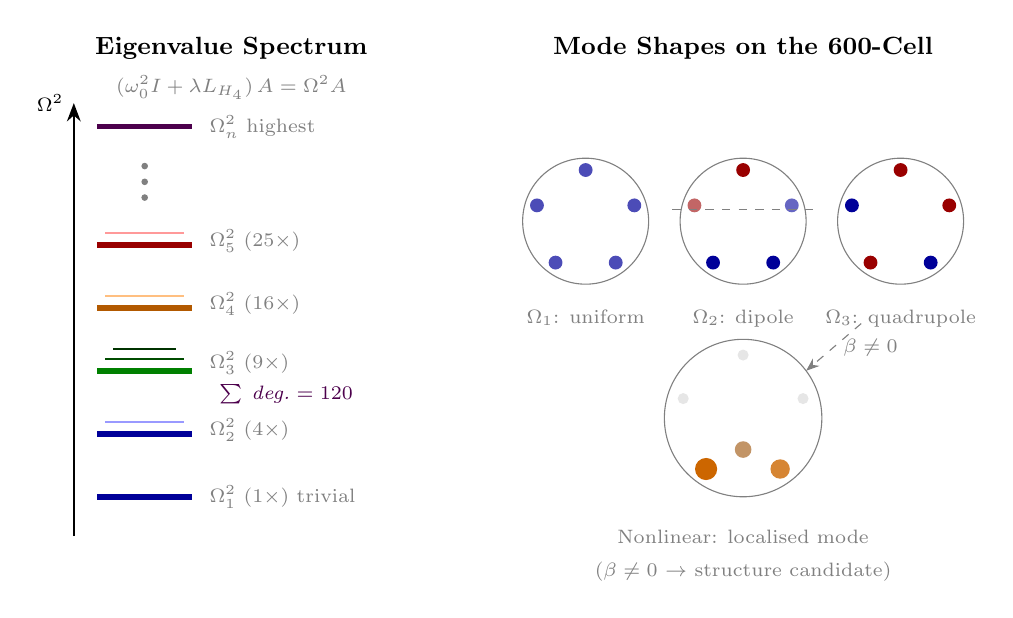
\begin{tikzpicture}[
    lbl/.style={font=\scriptsize, text=gray},
  ]

  % Left: spectrum
  \node[font=\small\bfseries] at (-3.5,4.2) {Eigenvalue Spectrum};
  \node[font=\scriptsize, text=gray] at (-3.5,3.7)
    {$(\omega_0^2 I + \lambda\Lmat)\,A = \Omega^2 A$};

  % Axis
  \draw[thick, -{Stealth}] (-5.5,-2) -- (-5.5,3.5)
    node[left, font=\scriptsize] {$\Omega^2$};

  % Levels
  \draw[blue!60!black, line width=2pt] (-5.2,-1.5) -- (-4.0,-1.5);
  \node[lbl, right] at (-3.9,-1.5) {$\Omega_1^2$ (1$\times$) trivial};

  \draw[blue!60!black, line width=2pt] (-5.2,-0.7) -- (-4.0,-0.7);
  \draw[blue!40, line width=1pt] (-5.1,-0.55) -- (-4.1,-0.55);
  \node[lbl, right] at (-3.9,-0.65) {$\Omega_2^2$ (4$\times$)};

  \draw[green!50!black, line width=2pt] (-5.2,0.1) -- (-4.0,0.1);
  \draw[green!30!black, line width=1pt] (-5.1,0.25) -- (-4.1,0.25);
  \draw[green!20!black, line width=0.7pt] (-5.0,0.38) -- (-4.2,0.38);
  \node[lbl, right] at (-3.9,0.2) {$\Omega_3^2$ (9$\times$)};

  \draw[orange!70!black, line width=2pt] (-5.2,0.9) -- (-4.0,0.9);
  \draw[orange!50, line width=1pt] (-5.1,1.05) -- (-4.1,1.05);
  \node[lbl, right] at (-3.9,0.95) {$\Omega_4^2$ (16$\times$)};

  \draw[red!60!black, line width=2pt] (-5.2,1.7) -- (-4.0,1.7);
  \draw[red!40, line width=1pt] (-5.1,1.85) -- (-4.1,1.85);
  \node[lbl, right] at (-3.9,1.75) {$\Omega_5^2$ (25$\times$)};

  \foreach \y in {2.3,2.5,2.7} {
    \fill[gray] (-4.6,\y) circle (1.2pt);
  }

  \draw[violet!60!black, line width=2pt] (-5.2,3.2) -- (-4.0,3.2);
  \node[lbl, right] at (-3.9,3.2) {$\Omega_n^2$ highest};

  \node[font=\scriptsize\itshape, text=violet!60!black]
    at (-2.8,-0.2) {$\sum$ deg.${}=120$};

  % Right: mode shapes
  \node[font=\small\bfseries] at (3,4.2) {Mode Shapes on the 600-Cell};

  % Mode 1: uniform
  \begin{scope}[shift={(1,2)}]
    \draw[gray, thin] (0,0) circle (0.8cm);
    \foreach \a in {90,162,234,306,378} {
      \fill[blue!60!black, opacity=0.7] (\a:0.65) circle (2.5pt);
    }
    \node[lbl, below] at (0,-1) {$\Omega_1$: uniform};
  \end{scope}

  % Mode 2: dipole
  \begin{scope}[shift={(3,2)}]
    \draw[gray, thin] (0,0) circle (0.8cm);
    \fill[red!60!black] (90:0.65) circle (2.5pt);
    \fill[red!60!black, opacity=0.6] (162:0.65) circle (2.5pt);
    \fill[blue!60!black] (234:0.65) circle (2.5pt);
    \fill[blue!60!black] (306:0.65) circle (2.5pt);
    \fill[blue!60!black, opacity=0.6] (378:0.65) circle (2.5pt);
    \draw[gray, dashed, thin] (-0.9,0.15) -- (0.9,0.15);
    \node[lbl, below] at (0,-1) {$\Omega_2$: dipole};
  \end{scope}

  % Mode 3: quadrupole
  \begin{scope}[shift={(5,2)}]
    \draw[gray, thin] (0,0) circle (0.8cm);
    \fill[red!60!black] (90:0.65) circle (2.5pt);
    \fill[blue!60!black] (162:0.65) circle (2.5pt);
    \fill[red!60!black] (234:0.65) circle (2.5pt);
    \fill[blue!60!black] (306:0.65) circle (2.5pt);
    \fill[red!60!black] (378:0.65) circle (2.5pt);
    \node[lbl, below] at (0,-1) {$\Omega_3$: quadrupole};
  \end{scope}

  % Mode n: localised (nonlinear)
  \begin{scope}[shift={(3,-0.5)}]
    \draw[gray, thin] (0,0) circle (1cm);
    \fill[gray, opacity=0.2] (90:0.8) circle (2pt);
    \fill[gray, opacity=0.2] (162:0.8) circle (2pt);
    \fill[orange!80!black] (234:0.8) circle (4pt);
    \fill[orange!80!black, opacity=0.8] (306:0.8) circle (3.5pt);
    \fill[gray, opacity=0.2] (378:0.8) circle (2pt);
    \fill[orange!60!black, opacity=0.6] (270:0.4) circle (3pt);
    \node[lbl, below] at (0,-1.3)
      {Nonlinear: localised mode};
    \node[lbl, below] at (0,-1.7)
      {($\beta \ne 0$ $\to$ structure candidate)};
  \end{scope}

  % Arrow linear -> nonlinear
  \draw[-{Stealth}, dashed, gray]
    (4.5,0.7) -- (3.8,0.1)
    node[midway, right, font=\scriptsize] {$\beta\ne 0$};

\end{tikzpicture}
\caption{Schematic of the eigenmode spectrum on the 600-cell graph.
\textit{Left:} the eigenvalue spectrum $\Omega^2$ is discrete and highly
degenerate due to $\Hfour$ symmetry.  \textit{Right:} low-lying eigenmodes
have simple spatial patterns (uniform, dipolar, quadrupolar); the nonlinear
regime ($\beta \ne 0$) permits localised structures that are candidates for
particle-like configurations.}
\label{fig:modes}
\end{figure}


% ══════════════════════════════════════════════════════════
\section{Numerical Validation of Dynamics}\label{sec:numerics}
% ══════════════════════════════════════════════════════════

% ── 7.1 ──────────────────────────────────────────────────
\subsection{Simulation Setup}

To investigate the dynamical consequences of the $\Hfour$-constrained
field equation~\eqref{eq:vfd}, numerical simulations were performed on
the 600-cell graph and compared against control graphs.

The following systems were considered:
\begin{itemize}[nosep]
\item \textbf{600-cell graph} (exact $\Hfour$ symmetry),
\item \textbf{Rewired control} (degree-preserving randomisation),
\item \textbf{Random 12-regular graph}.
\end{itemize}

The nonlinear oscillator system~\eqref{eq:vfd} was integrated using a
symplectic velocity--Verlet time-stepping scheme to preserve Hamiltonian
structure.  Energy conservation was verified to within $10^{-3}$ relative
error across all runs.  The nonlinear behaviour described here is
characteristic of coupled oscillator systems on graphs and does not
rely on any specific physical interpretation.

% ── 7.2 ──────────────────────────────────────────────────
\subsection{Localisation and Inverse Participation Ratio}

Localisation was quantified using the inverse participation ratio (IPR),
defined by
\begin{equation}\label{eq:ipr}
  \mathrm{IPR}(t) = \frac{\sum_i \Phi_i(t)^4}
                          {\left(\sum_i \Phi_i(t)^2\right)^2}.
\end{equation}

Across all tested regimes the 600-cell exhibits significantly higher
localisation than control graphs.  Averaged over long simulations:

\begin{table}[H]
\centering
\begin{tabular}{@{}lc@{}}
\toprule
System & Mean IPR \\
\midrule
600-cell ($\Hfour$)  & $\approx 0.15$ \\
Rewired control      & $\approx 0.03$ \\
Random 12-regular    & $\approx 0.03$ \\
\bottomrule
\end{tabular}
\caption{Mean IPR across long-time simulations.  The $\Hfour$ geometry
produces approximately $5\times$ stronger localisation than
degree-matched controls.}
\label{tab:ipr}
\end{table}

\begin{figure}[H]
\centering

\includegraphics[width=0.9\textwidth]{experiment/IPR_long_run.png}
\caption{IPR comparison between the 600-cell graph and control
graphs over long integration time.}
\label{fig:ipr_long}
\end{figure}

% ── 7.3 ──────────────────────────────────────────────────
\subsection{Spectral Sector Confinement}

Projection of the evolving field onto Laplacian eigenmodes reveals that
energy remains confined to a small number of spectral sectors in the
600-cell system.  In contrast, control graphs exhibit rapid diffusion
across the full eigenspectrum.  This difference is reflected in the
spectral entropy:
\begin{equation}\label{eq:spectral_entropy}
  S(t) = -\sum_k p_k(t)\log p_k(t),
\end{equation}
where $p_k(t)$ is the fraction of energy in sector~$k$.  The entropy
remains low (${\sim}\,1.5$~nats) for the 600-cell and significantly
higher (${\sim}\,3.5$~nats) for control systems.

\begin{figure}[H]
\centering

\includegraphics[width=0.9\textwidth]{experiment/spectral_entropy.png}
\caption{Spectral entropy comparison.  The 600-cell maintains
significantly lower entropy, indicating stronger spectral
confinement of the dynamics.}
\label{fig:spectral_entropy}
\end{figure}

\begin{figure}[H]
\centering

\includegraphics[width=0.9\textwidth]{experiment/spectral_band_evolution.png}
\caption{Spectral sector energy evolution.  Energy remains confined
to degenerate eigenvalue sectors on the 600-cell but spreads
uniformly for the control graph.}
\label{fig:spectral_bands}
\end{figure}

To separate spectral effects from geometric effects, isospectral
surrogate Laplacians were constructed preserving the eigenvalue spectrum
of the 600-cell while randomising the eigenvector basis.  Robust
breather-like localisation events appear only when the degenerate sector
structure is preserved, demonstrating that the dynamics depend on the
invariant eigenspace decomposition induced by $\Hfour$ symmetry rather
than on the spectrum alone.  This suggests that the dynamics are
governed not only by the eigenvalue spectrum but by the specific
arrangement of eigenvectors into symmetry-constrained sectors.

\begin{figure}[H]
\centering

\includegraphics[width=0.9\textwidth]{experiment/ipr_isospectral_comparison.png}
\caption{IPR comparison with isospectral surrogates.  The full
surrogate (random geometry, same spectrum) shows intermediate
localisation; the block surrogate (preserved sector structure)
matches the 600-cell exactly.}
\label{fig:ipr_iso}
\end{figure}

% ── 7.4 ──────────────────────────────────────────────────
\subsection{Shell Reflection and Distance-Regular Dynamics}

The 600-cell graph admits a symmetric partition of vertices into
distance shells around any origin vertex:
\begin{equation}\label{eq:shells}
  (1,\;12,\;32,\;42,\;32,\;1).
\end{equation}
Numerical results show coherent propagation of energy between shells,
with strong recurrence between the origin ($d=0$) and antipodal shell
($d=5$).  The shell cross-correlation between these sites reaches
${\sim}\,0.68$, compared to ${\sim}\,0.1$ for control graphs.  This
behaviour is consistent with a finite resonant cavity structure induced by the
distance-regular geometry of the 600-cell graph.

\begin{figure}[H]
\centering

\includegraphics[width=0.9\textwidth]{experiment/shell_reflection_map.png}
\caption{Shell energy propagation maps.  The 600-cell (top) shows
coherent vertical striping indicating recurrent energy return to
the origin.  The control (bottom) shows static horizontal bands
with no reflection structure.}
\label{fig:shell_map}
\end{figure}

\begin{figure}[H]
\centering

\includegraphics[width=0.9\textwidth]{experiment/shell_phase_correlation.png}
\caption{Cross-correlation between origin and antipodal shell
energies.  The 600-cell exhibits strong periodic correlation;
the controls show weak, irregular correlation.}
\label{fig:shell_corr}
\end{figure}

% ── 7.5 ──────────────────────────────────────────────────
\subsection{Spectral Beat Mechanism}

The recurrence behaviour observed in the 600-cell system can be
explained in terms of spectral beat frequencies.  The $\Hfour$ Laplacian
spectrum contains only nine distinct eigenvalues, yielding
\begin{equation}\label{eq:beats}
  \binom{9}{2} = 36
\end{equation}
distinct frequency gaps.  In contrast, control graphs with
${\sim}\,120$ distinct eigenvalues produce over $7\,000$ beat
frequencies.

The reduced number of frequencies in the 600-cell system allows for
constructive interference and periodic re-localisation of energy,
whereas the dense spectrum of the control graphs leads to destructive
interference and diffusion.  This provides a dynamical mechanism linking
spectral compression to persistent localisation.

The recurrence observed in the 600-cell system is therefore not a
nonlinear anomaly, but a direct consequence of the finite spectral
algebra induced by the $\Hfour$ symmetry.

\begin{figure}[H]
\centering

\includegraphics[width=0.9\textwidth]{experiment/ipr_recurrence_vs_spectrum.png}
\caption{IPR power spectrum compared with predicted spectral gap
frequencies.  The 600-cell shows sharp discrete peaks aligning
with the predicted gaps; the control shows a broad, featureless
spectrum.}
\label{fig:ipr_vs_gaps}
\end{figure}

\begin{figure}[H]
\centering

\includegraphics[width=0.9\textwidth]{experiment/gap_density_comparison.png}
\caption{Distribution of frequency gaps.  The 600-cell produces 36
discrete gaps from 9 sectors; the control produces over 7000 gaps
forming a near-continuous distribution.}
\label{fig:gap_density}
\end{figure}


% ══════════════════════════════════════════════════════════
\section{Relationship to \texorpdfstring{$\Eeight$}{E8} Symmetry}
\label{sec:e8}
% ══════════════════════════════════════════════════════════

% ── 7.1 ──────────────────────────────────────────────────
\subsection{The \texorpdfstring{$\Eeight$}{E8} Root System}

The $\Eeight$ lattice is an eight-dimensional lattice with exceptional
properties~\cite{conway1999e8}.  Its root system consists of 240~vectors of
minimal length, forming the vertices of the Gosset polytope~$4_{21}$.  The
$\Eeight$ lattice is the densest sphere packing in eight
dimensions~\cite{viazovska2017} and plays a central role in string theory,
where the gauge group $\Eeight \times \Eeight$ appears in the heterotic
string~\cite{gross1985}.

% ── 7.2 ──────────────────────────────────────────────────
\subsection{\texorpdfstring{$\Hfour$}{H4} Inside \texorpdfstring{$\Eeight$}{E8}}

A key mathematical relationship connects the $\Hfour$ and $\Eeight$ root
systems.  The $\Eeight$ root system admits a decomposition into two $\Hfour$ root
systems under a specific embedding into~$\R^8$~\cite{moody1984,sadoc1999}:
\begin{equation}\label{eq:e8_decomp}
  \Eeight\text{ roots (240)}
  \;\supset\;
  \Hfour\text{ roots (120)}
  \;\cup\;
  \Hfour'\text{ roots (120)}.
\end{equation}
This decomposition arises from a specific embedding of the $\Hfour$ root
system into~$\R^8$.  The two $\Hfour$ copies are related by a rotation in the
eight-dimensional space and together generate the full $\Eeight$ root system.
Certain projections of the $\Eeight$ root system onto four-dimensional
subspaces produce configurations with $\Hfour$
symmetry~\cite{moody1984}.

More precisely, there exists an orthogonal decomposition
$\R^8 = V_1 \oplus V_2$ where each $V_i \cong \R^4$, such that the projection
of the $\Eeight$ roots onto each four-dimensional subspace yields a copy of
the $\Hfour$ root system.  This is related to the Coxeter plane projection and
the ``golden ratio'' embedding studied by several
authors~\cite{sadoc1999,chen1998}.

% ── 7.3 ──────────────────────────────────────────────────
\subsection{Implications for VFD}

Within the VFD framework the $\Eeight \to \Hfour$ relationship suggests a
possible hierarchy of models:

\begin{description}[nosep, leftmargin=1.5cm, style=nextline]
  \item[Level 1] (this paper):\;
    A single $\Hfour$ system with 120~field sites on the 600-cell.  This is
    the minimal model and is sufficient to establish the basic eigenmode
    spectrum and structure formation mechanism.

  \item[Level 2] (future work):\;
    Two coupled $\Hfour$ systems, each carrying a 120-site field, embedded
    within an $\Eeight$ structure.  The coupling between the two $\Hfour$
    sectors would be governed by the eight-dimensional geometry and could give
    rise to additional structure: splitting of degenerate modes, inter-sector
    resonances, and new classes of coupled states.

  \item[Level 3] (speculative):\;
    A field defined on the full $\Eeight$ root system, with the $\Hfour$
    decomposition providing a natural basis for analysis.
\end{description}

It is important to emphasise that the $\Eeight$ connection is \emph{not
required} for the basic VFD framework presented in this paper.  The single
$\Hfour$ system on the 600-cell is self-contained and produces a well-defined
eigenmode spectrum.  The $\Eeight$ lattice is introduced here as a
\emph{possible higher-dimensional embedding} that may become relevant in future
extensions of the theory, not as a necessary ingredient of the present model.

% ── 7.4 ──────────────────────────────────────────────────
\subsection{Relation to Physics}

The appearance of $\Eeight$ in both string theory and the VFD symmetry ladder
raises the question of whether a deeper connection exists.  In heterotic string
theory the $\Eeight \times \Eeight$ gauge symmetry is a consequence of anomaly
cancellation in ten-dimensional supergravity~\cite{gross1985}.  In the VFD
context $\Eeight$ appears through the purely geometric route of polytope
symmetry extension.

Whether these two appearances of $\Eeight$ are related---or whether the VFD
geometric framework can make contact with established physical theories through
the $\Eeight$ connection---remains an open question.  We note the coincidence
without claiming a specific relationship.


% ══════════════════════════════════════════════════════════
\section{Implications}\label{sec:implications}
% ══════════════════════════════════════════════════════════

The framework developed in the preceding sections has several potential
consequences, which we outline here as directions for investigation rather than
as established results.

% ── 8.1 ──────────────────────────────────────────────────
\subsection{Discrete Structure Spectrum}

The eigenmode spectrum of the $\Hfour$ graph Laplacian produces a finite,
discrete set of allowed resonance frequencies and spatial configurations.  If the VFD mechanism were physically realised, this discreteness would
be consistent with the observed discreteness of particle species: only
those configurations corresponding to stable eigenmodes (or nonlinear
descendants thereof) would persist.  No direct mapping to known particle
spectra is assumed in the present work.

As computed in Section~\ref{sec:spectrum}, the 600-cell graph Laplacian
possesses exactly nine distinct eigenvalues with a highly organised
multiplicity structure (Table~\ref{tab:spectrum}).  The compressed spectral
hierarchy---nine resonance sectors spanning 120~degrees of freedom---suggests
that the $\Hfour$ geometry naturally organises the field into a small number of
collective mode families rather than an arbitrary collection of oscillatory
states.  This compression is a prerequisite for any resonance-based model
aiming to reproduce the observed finiteness of the particle spectrum.

% ── 8.2 ──────────────────────────────────────────────────
\subsection{Stability Hierarchy}

Not all eigenmodes are equally stable under perturbation.  In the nonlinear
regime some modes may be robust attractors while others are unstable saddle
configurations.  The stability hierarchy among the eigenmodes could provide an
ordering of structures by persistence---potentially analogous to the observed
hierarchy of particle lifetimes, where stable particles correspond to deeply
stable modes and short-lived resonances correspond to marginally stable
configurations.

% ── 8.3 ──────────────────────────────────────────────────
\subsection{Symmetry Constraints on Interactions}

The $\Hfour$ symmetry imposes selection rules on mode coupling.  Not all pairs
of modes can exchange energy through the cubic nonlinearity; the coupling is
governed by the representation-theoretic decomposition of tensor products.
These selection rules constrain the allowed ``interactions'' between
structure-modes in a manner reminiscent of conservation laws in particle
physics, though the specific content of these constraints has not yet been
computed for the $\Hfour$ system.

% ── 8.4 ──────────────────────────────────────────────────
\subsection{Dimensional Considerations}

The VFD field is defined on a four-dimensional symmetry manifold (the 600-cell
in~$\R^4$), while observable physics takes place in $3{+}1$ spacetime
dimensions.  The relationship between the internal symmetry dimensions of the
VFD framework and physical spacetime dimensions is not addressed in the
present work and represents a significant open question.  Possible approaches
include interpreting the $\Hfour$ manifold as an internal symmetry space
(analogous to Kaluza--Klein compactification) or as a constraint surface
embedded in a higher-dimensional space.

% ── 9.5 ──────────────────────────────────────────────────
\subsection{Geometry-Induced Dynamical Structure}

The numerical results of Section~\ref{sec:numerics} demonstrate that the
$\Hfour$ geometry does not merely constrain static eigenmodes but actively
shapes the dynamical behaviour of the system.  In particular:
\begin{itemize}[nosep]
\item Spectral compression leads to a reduced set of beat frequencies,
\item Distance-regular structure enables coherent shell reflection,
\item Degenerate eigenspaces confine energy to invariant subspaces.
\end{itemize}
These features combine to produce persistent localisation and recurrence
that are absent in structurally similar but non-symmetric graphs.


% ══════════════════════════════════════════════════════════
\section{Future Work}\label{sec:future}
% ══════════════════════════════════════════════════════════

The numerical experiments reported in Section~\ref{sec:numerics}
demonstrate that the $\Hfour$ shell supports coherent nonlinear dynamics
driven by a combination of spectral compression and symmetry-induced
sector structure.  Further work will investigate the stability properties
of the observed breather-like localisation events, the algebraic
structure underlying the spectral laws identified in the present work,
and extensions of the model to higher-dimensional symmetry embeddings.
The results establish that the $\Hfour$ symmetry geometry produces a
highly structured and non-generic resonance spectrum, providing a
concrete foundation for further mathematical and dynamical investigation.

The following steps are necessary to develop the framework further into a
quantitative model.

% ── 9.1 ──────────────────────────────────────────────────
\subsection{Explicit Eigenmode Computation}

The $120 \times 120$ graph Laplacian of the 600-cell should be explicitly
constructed and diagonalised.  This requires:
\begin{enumerate}[nosep]
  \item Generating the 120~vertex coordinates of the 600-cell.
  \item Determining the adjacency matrix from the edge connectivity
    (nearest-neighbour criterion).
  \item Computing $\Lmat = 12I - A$.
  \item Diagonalising to obtain the eigenvalue spectrum $\{\mu_k\}$ and
    eigenvectors $\{A^{(k)}\}$.
  \item Analysing the degeneracy pattern and identifying the corresponding
    $\Hfour$ representations.
\end{enumerate}
This computation is straightforward numerically and would yield the first
concrete VFD prediction: the resonance spectrum of the $\Hfour$ symmetry
shell.

% ── 9.2 ──────────────────────────────────────────────────
\subsection{Numerical Simulation of the Nonlinear System}

The full nonlinear field equation should be integrated numerically for various
values of the parameters $(\omega_0, \lambda, \beta)$ and initial conditions.
Key questions include:
\begin{itemize}[nosep]
  \item What stable localised modes (discrete breathers) exist on the 600-cell
    graph?
  \item How does the stability landscape depend on the nonlinearity
    parameter~$\beta$?
  \item Are there attracting configurations that emerge from generic initial
    conditions?
\end{itemize}
Standard numerical methods for nonlinear lattice dynamics (symplectic
integrators, Newton--Raphson continuation methods) are directly
applicable~\cite{flach2008}.

% ── 9.3 ──────────────────────────────────────────────────
\subsection{Spectral Gap Analysis}

Detailed analysis of the spectral gap structure and its relationship to
the recurrence periods observed in the numerical simulations
(Section~\ref{sec:numerics}) would clarify the mechanism underlying the
persistent localisation.  The $36$~beat frequencies arising from the nine
Laplacian sectors provide a finite algebraic structure whose properties
may be amenable to exact analysis.  A key open problem is to derive the
observed Laplacian spectrum directly from the distance-regular
intersection array and associated Bose--Mesner algebra of the 600-cell
graph.

% ── 9.4 ──────────────────────────────────────────────────
\subsection{Representation-Theoretic Analysis}

A systematic decomposition of the 120-dimensional permutation representation
of $\Hfour$ into irreducible components would provide the complete
classification of eigenmodes and their coupling rules.  This analysis draws on
the well-studied representation theory of finite reflection
groups~\cite{broue2010}.

% ── 9.4 ──────────────────────────────────────────────────
\subsection{Mapping to Physical Observables}

If the eigenmode spectrum can be computed, the most important next step is to
determine whether any subset of the spectrum, or any ratio of eigenvalues,
corresponds to known physical quantities---such as particle mass ratios or
coupling constant relationships.  Such a correspondence, even if approximate,
would constitute significant evidence for the physical relevance of the
framework.

% ── 9.5 ──────────────────────────────────────────────────
\subsection{Extension to \texorpdfstring{$\Eeight$}{E8}}

As discussed in Section~\ref{sec:e8}, the two-$\Hfour$ model embedded in
$\Eeight$ represents a natural extension.  This would double the number of
field sites to~240 and introduce inter-sector coupling governed by the
eight-dimensional geometry.


% ══════════════════════════════════════════════════════════
% References
% ══════════════════════════════════════════════════════════
\newpage
\begin{thebibliography}{28}

\bibitem{noether1918}
E.~Noether,
``Invariante Variationsprobleme,''
\textit{Nachrichten von der Gesellschaft der Wissenschaften zu G\"ottingen},
pp.~235--257, 1918.

\bibitem{weinberg1996}
S.~Weinberg,
\textit{The Quantum Theory of Fields}, Vol.~II\@.
Cambridge University Press, 1996.

\bibitem{mtw1973}
C.~W.~Misner, K.~S.~Thorne, and J.~A.~Wheeler,
\textit{Gravitation}.
W.~H.~Freeman, 1973.

\bibitem{berry1984}
M.~V.~Berry,
``Quantal phase factors accompanying adiabatic changes,''
\textit{Proc.\ R.\ Soc.\ Lond.\ A}, vol.~392, pp.~45--57, 1984.

\bibitem{nakahara2003}
M.~Nakahara,
\textit{Geometry, Topology and Physics}, 2nd~ed.
CRC Press, 2003.

\bibitem{arkani2014}
N.~Arkani-Hamed and J.~Trnka,
``The Amplituhedron,''
\textit{J.\ High Energy Phys.}, vol.~2014, no.~10, p.~30, 2014.

\bibitem{humphreys1990}
J.~E.~Humphreys,
\textit{Reflection Groups and Coxeter Groups}.
Cambridge University Press, 1990.

\bibitem{conway1999}
J.~H.~Conway and N.~J.~A.~Sloane,
\textit{Sphere Packings, Lattices and Groups}, 3rd~ed.
Springer, 1999.

\bibitem{coxeter1973}
H.~S.~M.~Coxeter,
\textit{Regular Polytopes}, 3rd~ed.
Dover Publications, 1973.

\bibitem{coxeter1988}
H.~S.~M.~Coxeter,
``Regular and semi-regular polytopes, III,''
\textit{Math.\ Z.}, vol.~200, pp.~3--45, 1988.

\bibitem{mcmullen2002}
P.~McMullen and E.~Schulte,
\textit{Abstract Regular Polytopes}.
Cambridge University Press, 2002.

\bibitem{coxeter1991}
H.~S.~M.~Coxeter,
\textit{Regular Complex Polytopes}, 2nd~ed.
Cambridge University Press, 1991.

\bibitem{moody1993}
R.~V.~Moody and J.~Patera,
``Quasicrystals and icosians,''
\textit{J.\ Phys.\ A}, vol.~26, pp.~2829--2853, 1993.

\bibitem{conway2003}
J.~H.~Conway and D.~A.~Smith,
\textit{On Quaternions and Octonions}.
A.~K.~Peters, 2003.

\bibitem{wilson2009}
R.~A.~Wilson,
\textit{The Finite Simple Groups}.
Springer, 2009.

\bibitem{chung1997}
F.~R.~K.~Chung,
\textit{Spectral Graph Theory}.
AMS, 1997.

\bibitem{brouwer2012}
A.~E.~Brouwer and W.~H.~Haemers,
\textit{Spectra of Graphs}.
Springer, 2012.

\bibitem{vilenkin1993}
N.~J.~Vilenkin and A.~U.~Klimyk,
\textit{Representation of Lie Groups and Special Functions}, Vol.~2.
Kluwer Academic, 1993.

\bibitem{serre1977}
J.-P.~Serre,
\textit{Linear Representations of Finite Groups}.
Springer, 1977.

\bibitem{flach2008}
S.~Flach and A.~V.~Gorbach,
``Discrete breathers --- advances in theory and applications,''
\textit{Phys.\ Rep.}, vol.~467, pp.~1--116, 2008.

\bibitem{mackay1994}
R.~S.~MacKay and S.~Aubry,
``Proof of existence of breathers for time-reversible or Hamiltonian networks
of weakly coupled oscillators,''
\textit{Nonlinearity}, vol.~7, pp.~1623--1643, 1994.

\bibitem{conway1999e8}
J.~H.~Conway and N.~J.~A.~Sloane,
``The $E_8$ lattice,'' Chapter~8 in
\textit{Sphere Packings, Lattices and Groups}, 3rd~ed.
Springer, 1999.

\bibitem{viazovska2017}
M.~S.~Viazovska,
``The sphere packing problem in dimension~8,''
\textit{Ann.\ Math.}, vol.~185, pp.~991--1015, 2017.

\bibitem{gross1985}
D.~J.~Gross, J.~A.~Harvey, E.~Martinec, and R.~Rohm,
``Heterotic string theory~(I). The free heterotic string,''
\textit{Nucl.\ Phys.\ B}, vol.~256, pp.~253--284, 1985.

\bibitem{moody1984}
R.~V.~Moody and J.~Patera,
``Characters of elements of finite order in Lie groups,''
\textit{SIAM J.\ Algebraic Discrete Methods}, vol.~5, pp.~359--383, 1984.

\bibitem{sadoc1999}
J.~F.~Sadoc and R.~Mosseri,
\textit{Geometrical Frustration}.
Cambridge University Press, 1999.

\bibitem{chen1998}
B.~L.~Chen, R.~V.~Moody, and J.~Patera,
``Non-crystallographic root systems,'' in
\textit{Quasicrystals and Discrete Geometry},
Fields Institute Monographs, AMS, 1998.

\bibitem{broue2010}
M.~Brou\'e,
\textit{Introduction to Complex Reflection Groups and Their Braid Groups}.
Springer, 2010.

\end{thebibliography}


% ══════════════════════════════════════════════════════════
\appendix
\section{Numerical Construction of the 600-Cell Graph}
\label{app:construction}
% ══════════════════════════════════════════════════════════

This appendix describes the procedure used to construct the 600-cell graph and
compute the Laplacian spectrum reported in Section~\ref{sec:spectrum}.  All
steps are reproducible using standard numerical linear algebra software.

\subsection{Vertex Coordinates}

The 120~vertices of the 600-cell inscribed in the unit 3-sphere
$S^3 \subset \R^4$ were generated using the quaternion representation.  The
vertex set consists of the 120~unit quaternions forming the binary icosahedral
group~$2I$~\cite{conway2003}.  These can be constructed explicitly as the
union of the following sets (all permutations of coordinates and even sign
changes):

\begin{enumerate}[nosep]
  \item \textbf{8 vertices:} all permutations of $({\pm}1, 0, 0, 0)$.
  \item \textbf{16 vertices:} $\tfrac{1}{2}({\pm}1, {\pm}1, {\pm}1, {\pm}1)$
    (all sign combinations).
  \item \textbf{96 vertices:} all even permutations of
    $\tfrac{1}{2}(0, {\pm}1, {\pm}\vphi, {\pm}\hat\vphi)$,
    where $\vphi = \tfrac{1+\sqrt{5}}{2}$ and
    $\hat\vphi = \tfrac{1-\sqrt{5}}{2}$.
\end{enumerate}

\noindent These yield $8 + 16 + 96 = 120$ unit vectors in~$\R^4$.

\subsection{Adjacency Matrix}

Two vertices $v_i$ and $v_j$ are declared adjacent if and only if their
Euclidean distance equals the edge length of the 600-cell inscribed in the
unit sphere.  For a unit-radius 600-cell the edge length is
\begin{equation}\label{eq:edge_length}
  d_{\text{edge}} = \frac{1}{\vphi} = \vphi - 1 = \frac{\sqrt{5}-1}{2}
  \approx 0.6180.
\end{equation}
Equivalently, using the inner product, vertices $v_i$ and $v_j$ are adjacent
if
\begin{equation}\label{eq:adjacency_criterion}
  \langle v_i, v_j \rangle
  = 1 - \frac{d_{\text{edge}}^2}{2}
  = 1 - \frac{3 - \sqrt{5}}{4}
  = \frac{1 + \sqrt{5}}{4}
  = \frac{\vphi}{2}
  \approx 0.80902.
\end{equation}

In practice, adjacency is determined by checking whether
$\bigl|\langle v_i, v_j \rangle - \vphi/2\bigr| < \varepsilon$
for a small numerical tolerance~$\varepsilon$.  The resulting adjacency matrix~$A$ is a
$120 \times 120$ symmetric binary matrix with exactly $12$~ones in each row,
confirming the 12-regular structure.  The total number of edges is
$\tfrac{1}{2} \times 120 \times 12 = 720$, matching the known combinatorial
data for the 600-cell.

\subsection{Laplacian and Diagonalisation}

The graph Laplacian is computed as $\Lmat = 12I - A$.  Standard eigenvalue
decomposition (e.g.\ \texttt{numpy.linalg.eigh} or equivalent) yields
120~eigenvalues.  Grouping by numerical equality (within floating-point
tolerance) produces the nine distinct eigenvalues and multiplicities reported
in Table~\ref{tab:spectrum}.

The closed-form expressions for the irrational eigenvalues ($9 \pm 3\sqrt{5}$
and $10 \pm 2\sqrt{5}$) were identified by comparing the numerical values
against algebraic expressions in $\Q(\sqrt{5}\,)$ and verified to match within
machine precision.

Code used to generate the 600-cell graph and compute the Laplacian spectrum
will be released in a companion repository.

\subsection{Reproducibility}

All numerical experiments described in Section~\ref{sec:numerics} are
implemented in a companion code package (\texttt{vfd\_sim}), including:
\begin{itemize}[nosep]
\item graph construction and verification,
\item Laplacian diagonalisation,
\item nonlinear time evolution (symplectic integrator),
\item spectral and localisation diagnostics,
\item control graph generation and false-positive testing.
\end{itemize}

\vfill
\noindent\rule{\textwidth}{0.4pt}\\[4pt]
{\footnotesize
\textit{Vibrational Field Dynamics Working Paper Series}
\hfill WO-VFD-PAPER-001 \quad Draft v1.1 (submission-ready)}

\end{document}
